% ---------------------------- Preamble starts here ----------------------------

\documentclass[aspectratio=169]{beamer} %Remove [aspectratio=169] to get non-wide 4:3 slide aspect ratio

%-----------------------------------------------
% --- Set beamer theme
\usetheme{Metropolis}
\setbeamertemplate{footline}{}				% Remove automatic footer
\setbeamertemplate{navigation symbols}{}	% Comment this line to display navigation symbols

%-----------------------------------------------
% Load i2i symbol
\addtobeamertemplate{frametitle}{}{%
\begin{textblock*}{\linewidth}(0cm,7.4cm) % Replace with (0cm, 8cm) if using non-wide slide aspect
	
\includegraphics[width=\linewidth]{../../Common-Resources/img/Footer.png}
\end{textblock*}}

%-----------------------------------------------
% --- Load packages
\usepackage{textpos}		% To align objects correctly
\usepackage{multicol}		% To right in multiple columns
\usepackage{color}			% To color text

%-----------------------------------------------
% --- Include link to last commit
\usepackage{xstring}
\usepackage{catchfile}

%Set this user input
\newcommand{\gitfolder}{../../../.git} %relative path to .git folder from .tex doc
\newcommand{\reponame}{worldbank/dime-github-trainings} % Name of account and repo be set in URL

%Based on this https://tex.stackexchange.com/questions/455396/how-to-include-the-current-git-commit-id-and-branch-in-my-document
\CatchFileDef{\headfull}{\gitfolder/HEAD.}{} 				%Get path to head file for checked out branch
\StrGobbleRight{\headfull}{1}[\head]						%Remove end of line character
\StrBehind[2]{\head}{/}[\branch]							%Parse out the path only
\CatchFileDef{\commit}{\gitfolder/refs/heads/\branch.}{}	%Get the content of the branch head
\StrGobbleRight{\commit}{1}[\commithash]					%Remove end of line characted

%Build the URL to this commit based on the information we now have
\newcommand{\commiturl}{\url{https://github.com/\reponame/commit/\commithash}}

%-----------------------------------------------
% --- Add your information here
\title{GitHub - Pull Request training}
\author{DIME Analytics}
\institute{DIME - The World Bank - \trainingURL{https://www.worldbank.org/en/research/dime}}
\date{\today}

\newcommand{\trainingURL}[1]{{\color{blue}\url{#1}}}

\newcommand{\traininerUsername}{kbjarkefur}
\newcommand{\repoName}{\traininerUsername/lyrics}
\newcommand{\trainingRepoURL}[1]{\trainingURL{github.com/\repoName #1}}
\newcommand{\trainerEmail}{\trainingURL{kbjarkefur@worldbank.org} }


% ---------------------------- Preamble ends here ----------------------------

\begin{document}

\begin{frame}

\includegraphics[width=\textwidth]{../../Common-Resources/img/Header.png}
\vspace{-0.2cm}
\titlepage 	 % Opening slide, prints inform
\end{frame}

\begin{frame}
	\frametitle{Who is this training for}
	
	
	\begin{columns}[c]
		
		\column{.65\textwidth} % Left column and width

		\large \textbf{Who is this training for?}
		
		\vspace{1em}
		
		Anyone comfortable branching, committing and merging in Git/GitHub who is ready to be introduced to a more advanced workflow using Git/GitHub to ensure high quality code.		
		
		\column{.35\textwidth} % Left column and width
		
		ADD SOME ICON/PICTURE
		
	\end{columns}

\end{frame}

\begin{frame}
	\frametitle{Content}

	\Large\centering \textbf{THIS TRAINING HAS TWO PARTS}
	
	\vspace{.8em}
	
	\begin{columns}[T]
		
		\column{.08\textwidth}
		
		\column{.4\textwidth} % Left column and width

		\centering 
		\large \textbf{Part 1}

		\vspace{1em}
		
		\raggedright
		\normalfont Introducing a framework for the \textit{branch-PR-merge} cycle,
		and best practices for each step
		
		\vspace{.5em}
		
		\normalfont This framework should be used for 
		each task implemented on Git/GitHub
		
		\column{.04\textwidth}
		
		\column{.4\textwidth} % Left column and width
		
		\centering 
		\large \textbf{Part 2}
		
		\vspace{1em}
		
		\raggedright
		\normalfont How to integrate the \textit{branch-PR-merge} cycle for a typical DIME research project
		
		\vspace{.5em}
		
		\normalfont Intro to the GitFlow philosophy
		
		\column{.08\textwidth}
		
	\end{columns}
	
	\end{frame}



\section{Part 1: \newline Best practices for the branch-PR-merge cycle}

\begin{frame}
\frametitle{The branch-PR-merge cycle}

	\begin{columns}[c]
	
		\column{.35\textwidth} % Left column and width
		\large The branch-PR-merge cycle 
		\vspace{.7cm}\newline
		\large Complete this cycle for \textbf{all tasks}
		\vspace{.7cm}\newline
		\large We will go over all steps but focus today on the \textbf{work stage}	

		\column{.65\textwidth} % Right column and width
		\vspace{-.75cm}
		\begin{figure}
			\centering
			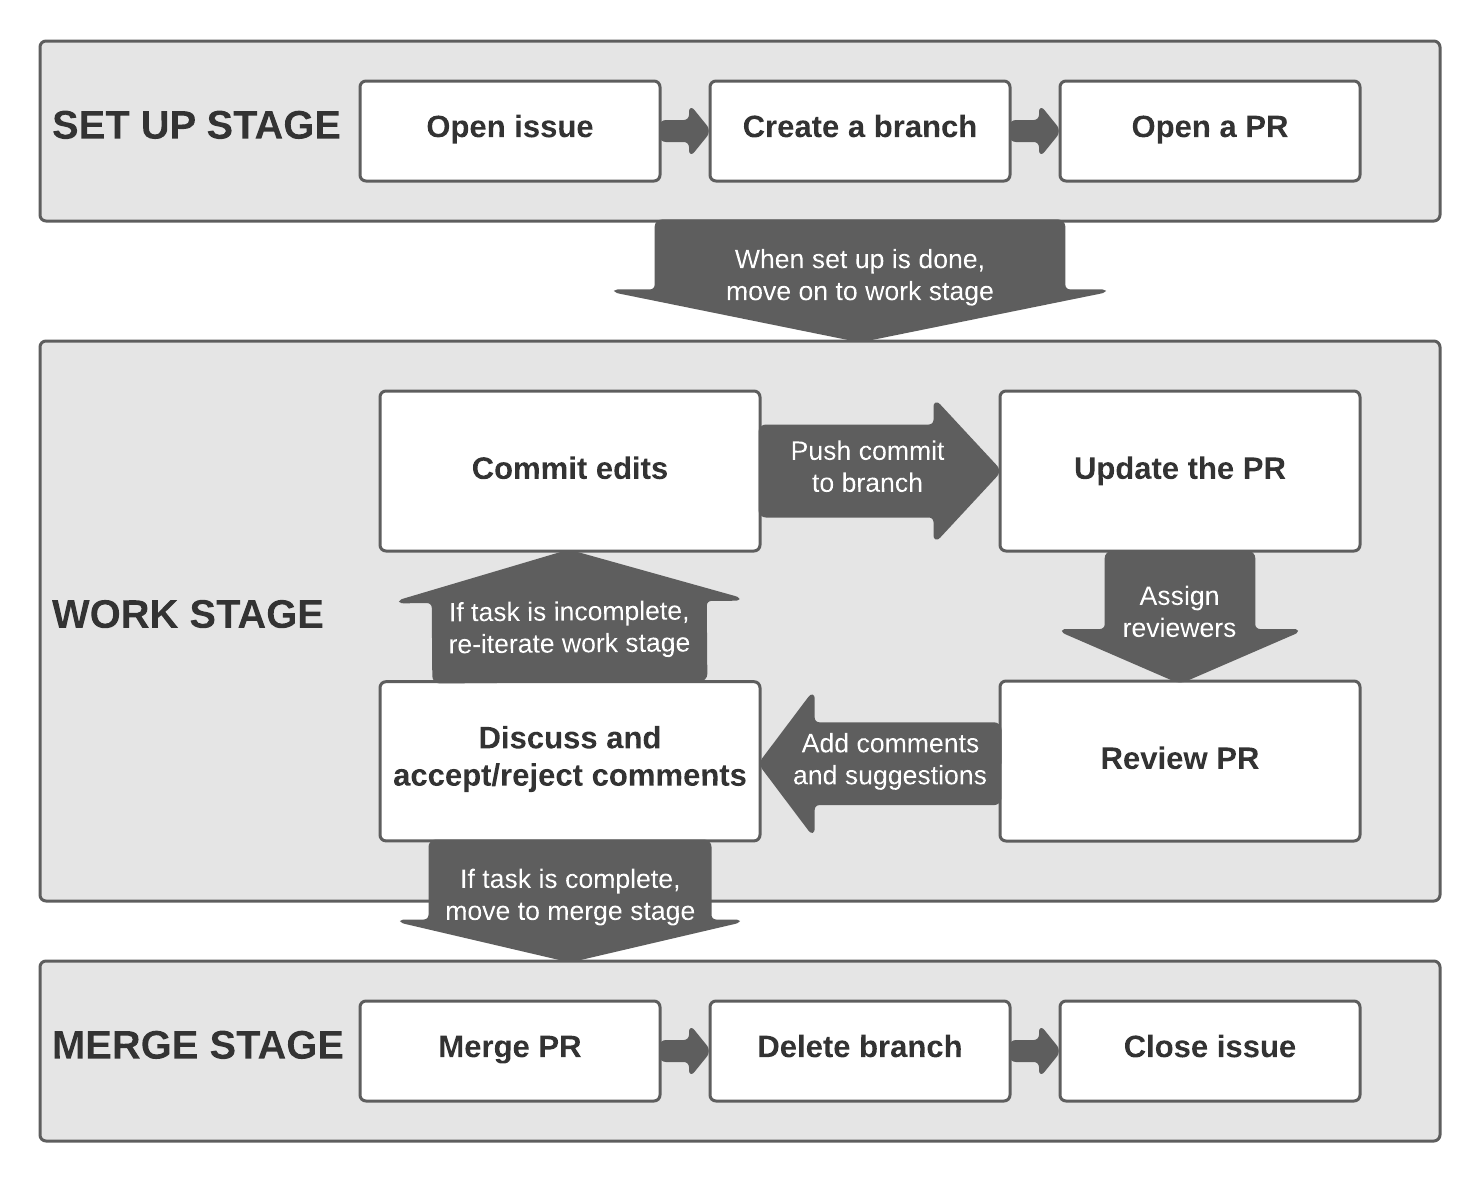
\includegraphics[width=\textwidth]{./img/branch-pr-merge-cycle.png}
		\end{figure}
		
	\end{columns}
\end{frame}

\begin{frame}
	\frametitle{Stage: The set up stage}
	
	\huge\centering \textbf{SET UP STAGE}
	
\end{frame}


\begin{frame}
	\frametitle{Stage: The set up stage}
	\begin{columns}[c]

		\column{.35\textwidth} % Left column and width
		
		\Large \textbf{The set up stage:}
		\vspace{1em}
		\normalsize
		
		\begin{itemize}
			\setlength\itemsep{1em}
			\item Document the task you will work on
			\item Create a space in your repo to work on the task
		\end{itemize}
		
		\column{.65\textwidth} % Right column and width
		\vspace{-.75cm}
		\begin{figure}
			\centering
			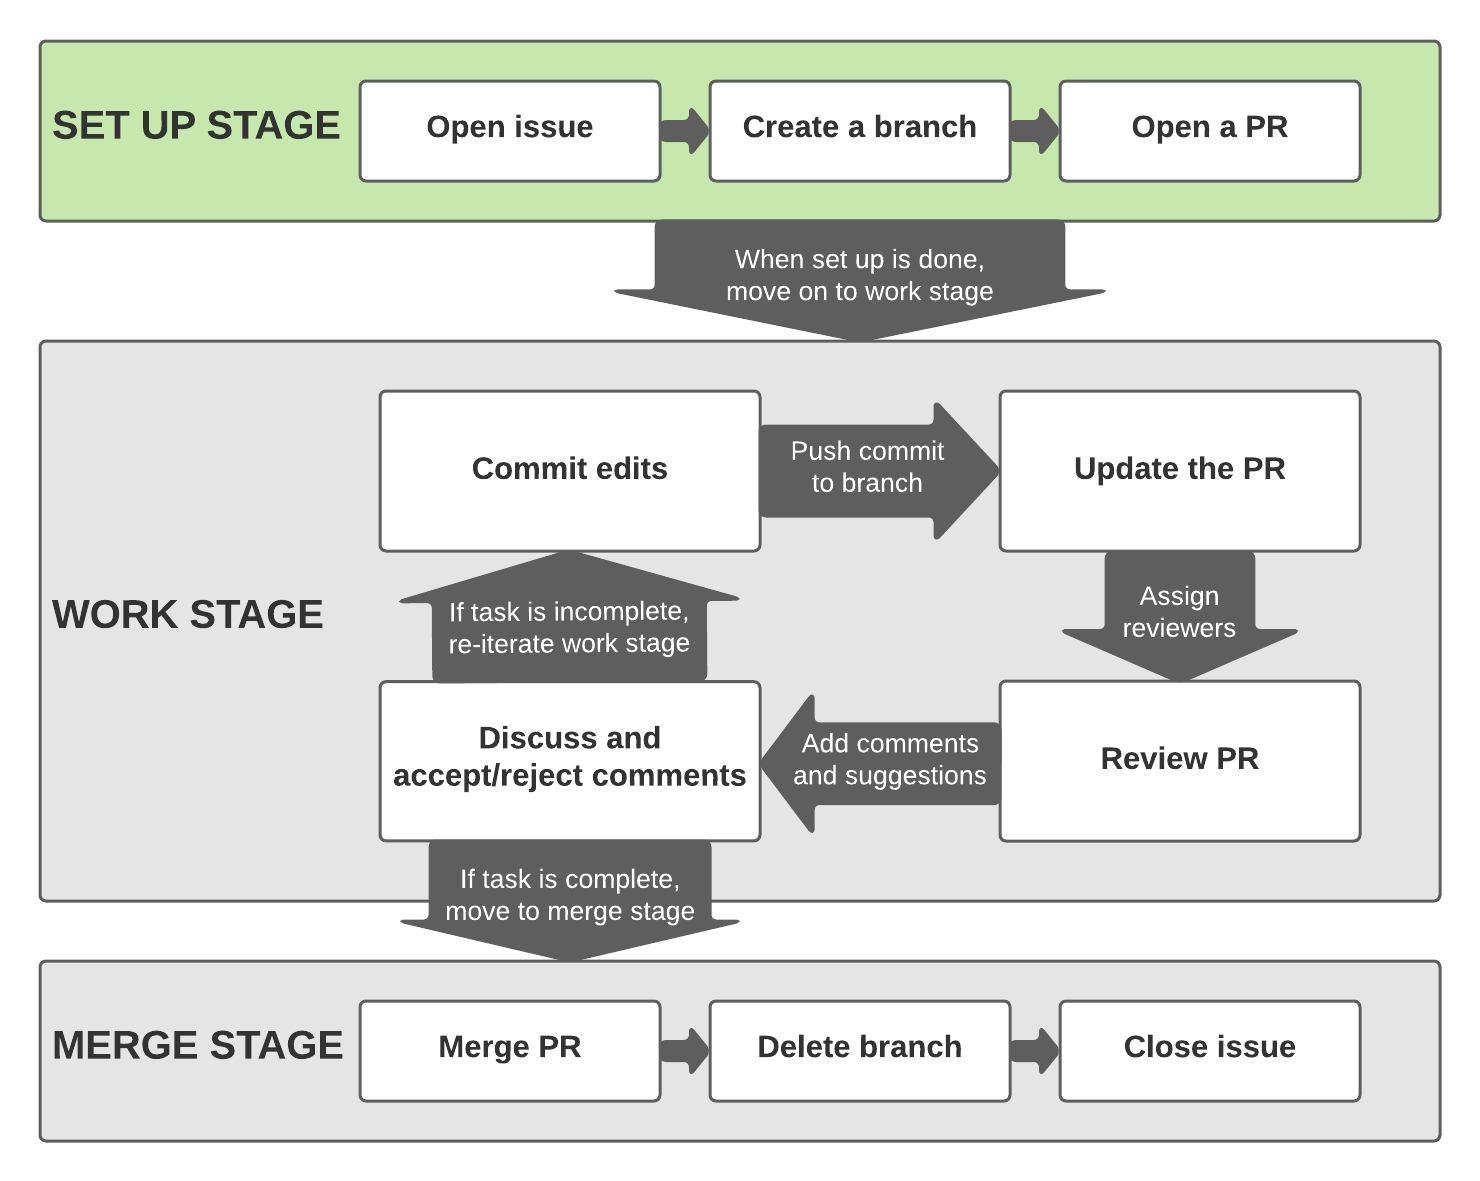
\includegraphics[width=\textwidth]{./img/branch-pr-merge-cycle-S1.png}
		\end{figure}
		
	\end{columns}
\end{frame}


\begin{frame}
	\frametitle{Step: Create an issue}
	\begin{columns}[c]
		
		\column{.35\textwidth} % Left column and width
		\begin{itemize}
			\setlength\itemsep{.5em}
			\item Issues is a great way to document what tasks need to be done
			\item Issues allow other team members to provide input on how to solve the task
			\item No need to open an issue for tasks that will be done immediately and has no need for a place to document discussions about the task
		\end{itemize}
		
		\column{.65\textwidth} % Right column and width
		\vspace{-.75cm}
		\begin{figure}
			\centering
			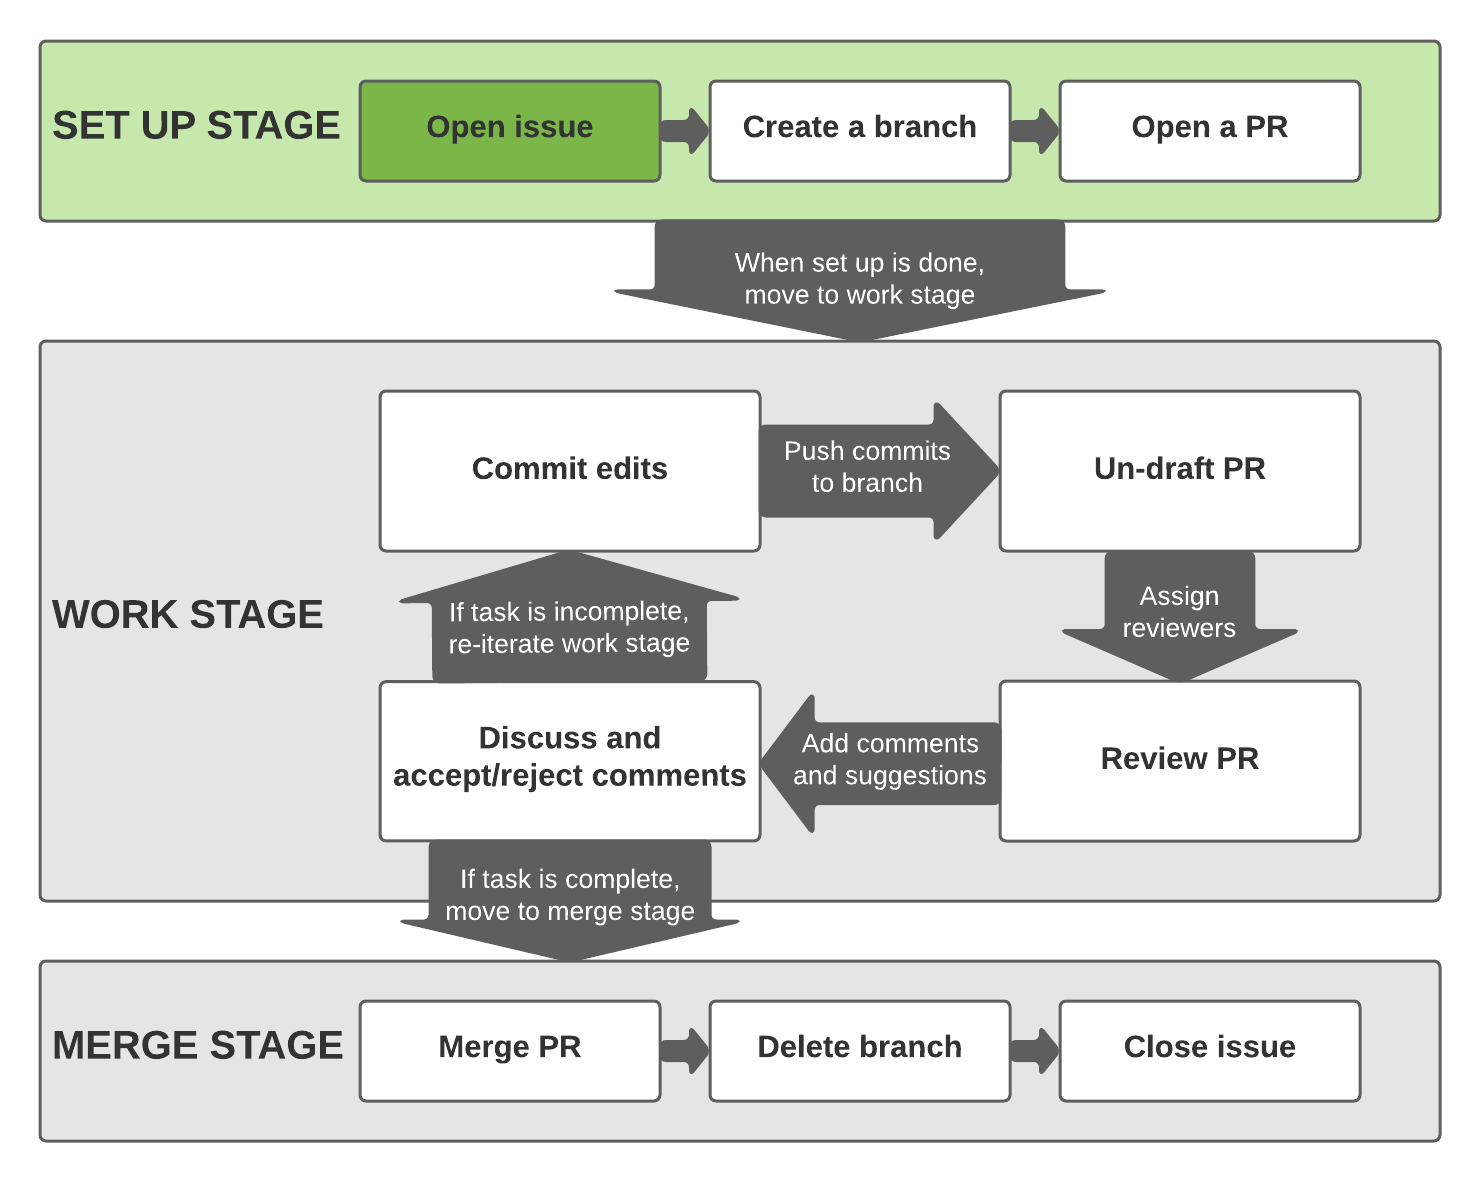
\includegraphics[width=\textwidth]{./img/branch-pr-merge-cycle-S1-1.png}
		\end{figure}
		
	\end{columns}
\end{frame}

\begin{frame}
	\frametitle{Create an issue}
	\begin{columns}[c]

		\column{.55\textwidth} % Right column and width
		\vspace{-.5cm}
		\begin{figure}
			\centering
			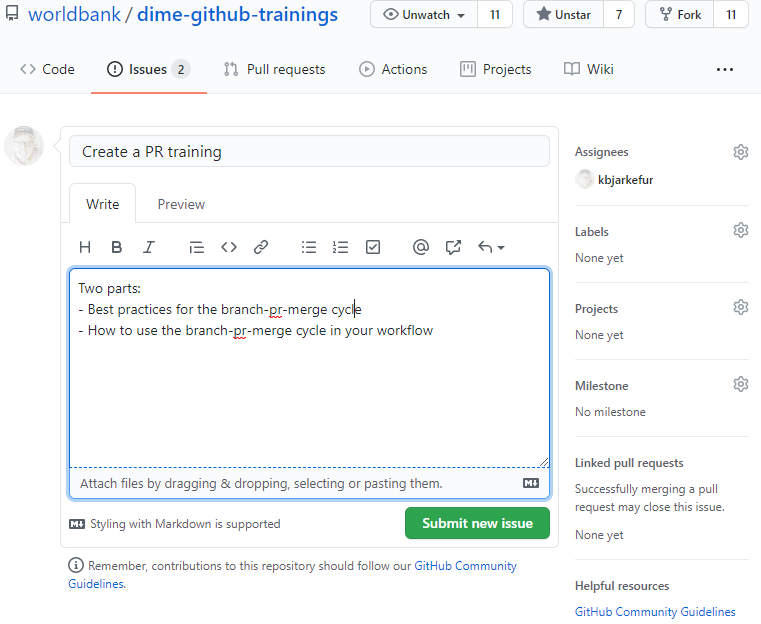
\includegraphics[width=\textwidth]{./img/create-issue-1.png}
		\end{figure}
		
		\column{.45\textwidth} % Left column and width
		
		\begin{itemize}
			\setlength\itemsep{.5em}
			\item Click the issues tab and then \texttt{New Issue}
			\item Document the task and/or ask the rest of the team of input
			\item Assign yourself or someone to complete the task
			\item Add labels to facilitate future searches
			\item This is far superior way to document tasks compared to emails or in-person meetings!
		\end{itemize}
			
	\end{columns}	
\end{frame}

\begin{frame}
	\frametitle{Browse an issue}
	\begin{columns}[c]
		
		\column{.55\textwidth} % Right column and width
		\vspace{-.5cm}
		\begin{figure}
			\centering
			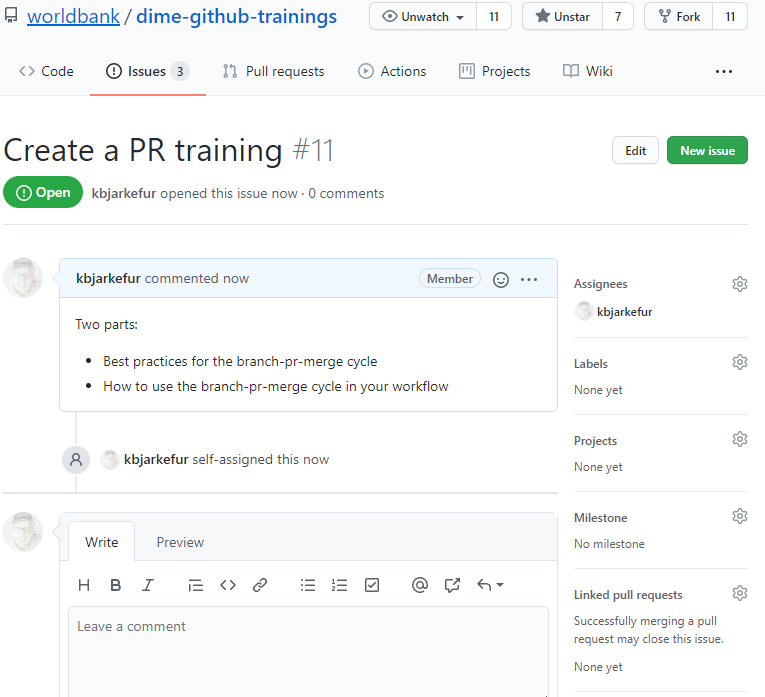
\includegraphics[width=\textwidth]{./img/create-issue-2.png}
		\end{figure}
		
		\column{.45\textwidth} % Left column and width
		
		\begin{itemize}
			\setlength\itemsep{1em}
			\item Take note of issue number (also found in URL) so you can refer to it
			\item Anyone can use the comment field to provide input
			\item You can update assignees and/or labels
			\item Even when closed, this issue may be browsed by future team members
		\end{itemize}
		
	\end{columns}	
\end{frame}

\begin{frame}
	\frametitle{Create a branch}
	\begin{columns}[c]
		
		\column{.35\textwidth} % Left column and width
		\begin{itemize}
			\setlength\itemsep{.5em}
			\item Create branch on GitHub.com
			\item We create a branch to create a space where work on this task does not interfere with work on other tasks
			\item Name it after the task and suffix name with issue number - for example: \texttt{pr-training-11}
		\end{itemize}
		
		\column{.65\textwidth} % Right column and width
		\vspace{-.75cm}
		\begin{figure}
			\centering
			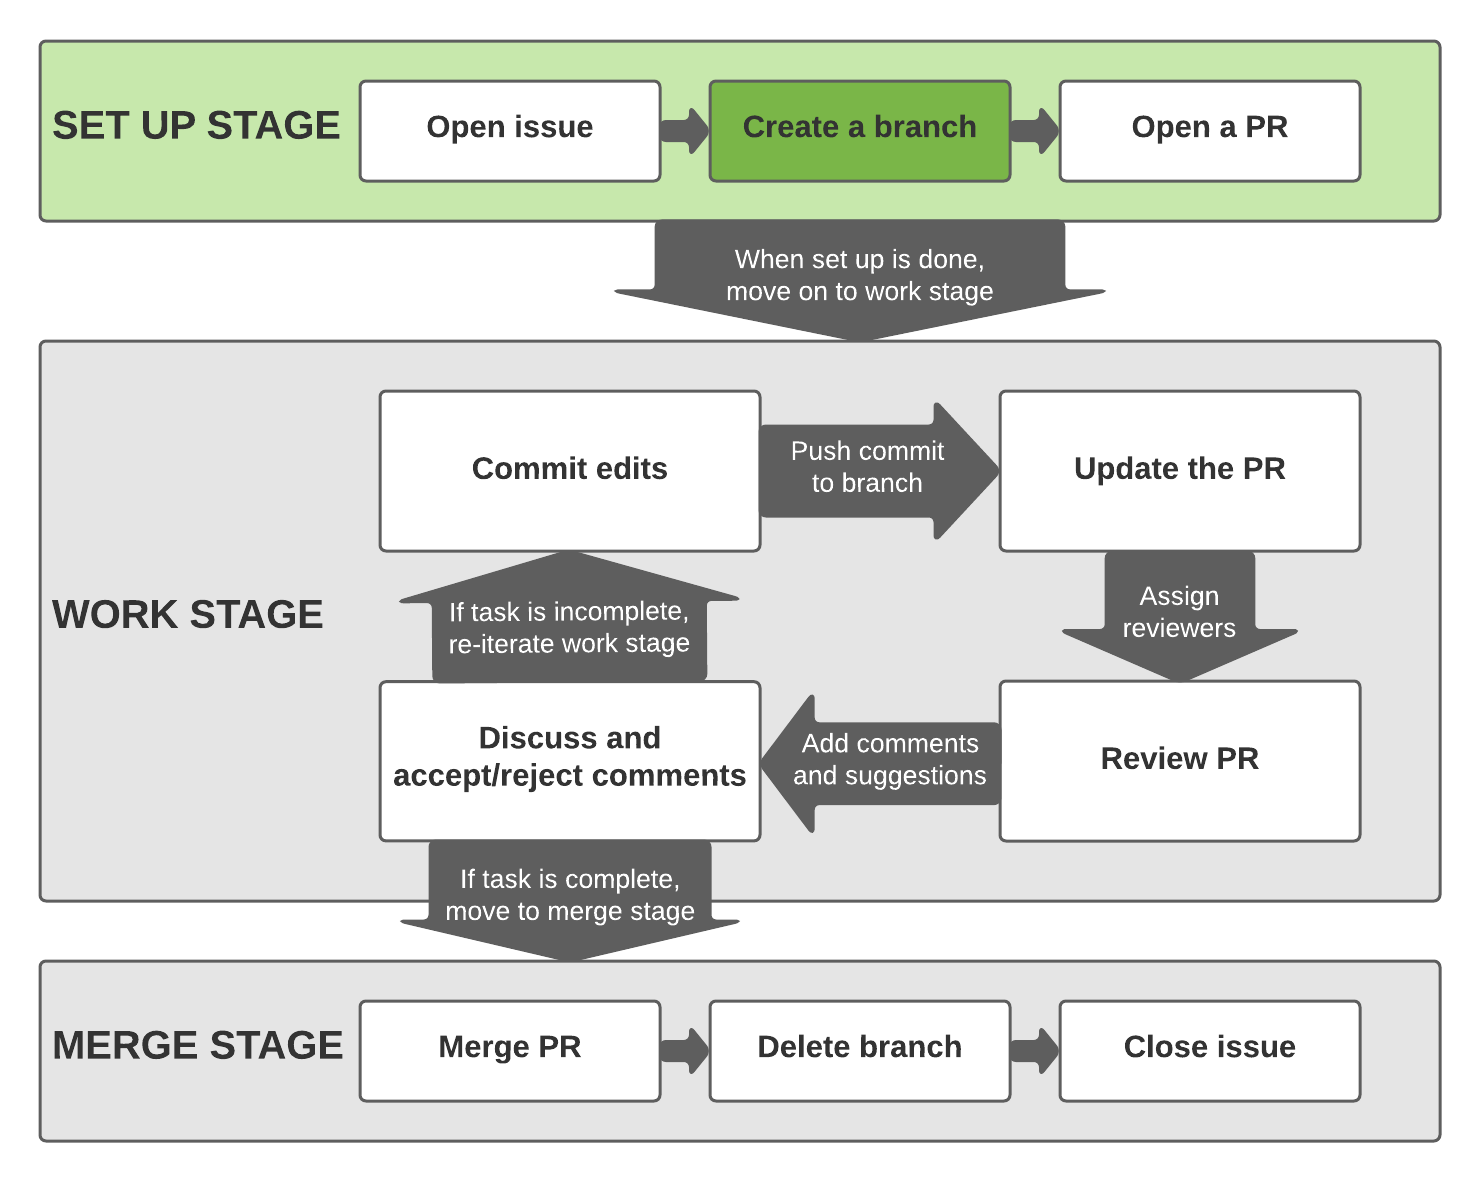
\includegraphics[width=\textwidth]{./img/branch-pr-merge-cycle-S1-2.png}
		\end{figure}
		
	\end{columns}
\end{frame}

\begin{frame}
	\frametitle{Open the PR}
	\begin{columns}[c]
		
		\column{.35\textwidth} % Left column and width
		\begin{itemize}
			\setlength\itemsep{1em}
			\item Create a PR \textbf{before} you start working - this creates a space on GitHub where the progress of this task can be followed
			\item Create a \textit{``draft PR''} for work in progress
			\item Reference branch name in PR name
		\end{itemize}
		
		\column{.65\textwidth} % Right column and width
		\vspace{-.75cm}
		\begin{figure}
			\centering
			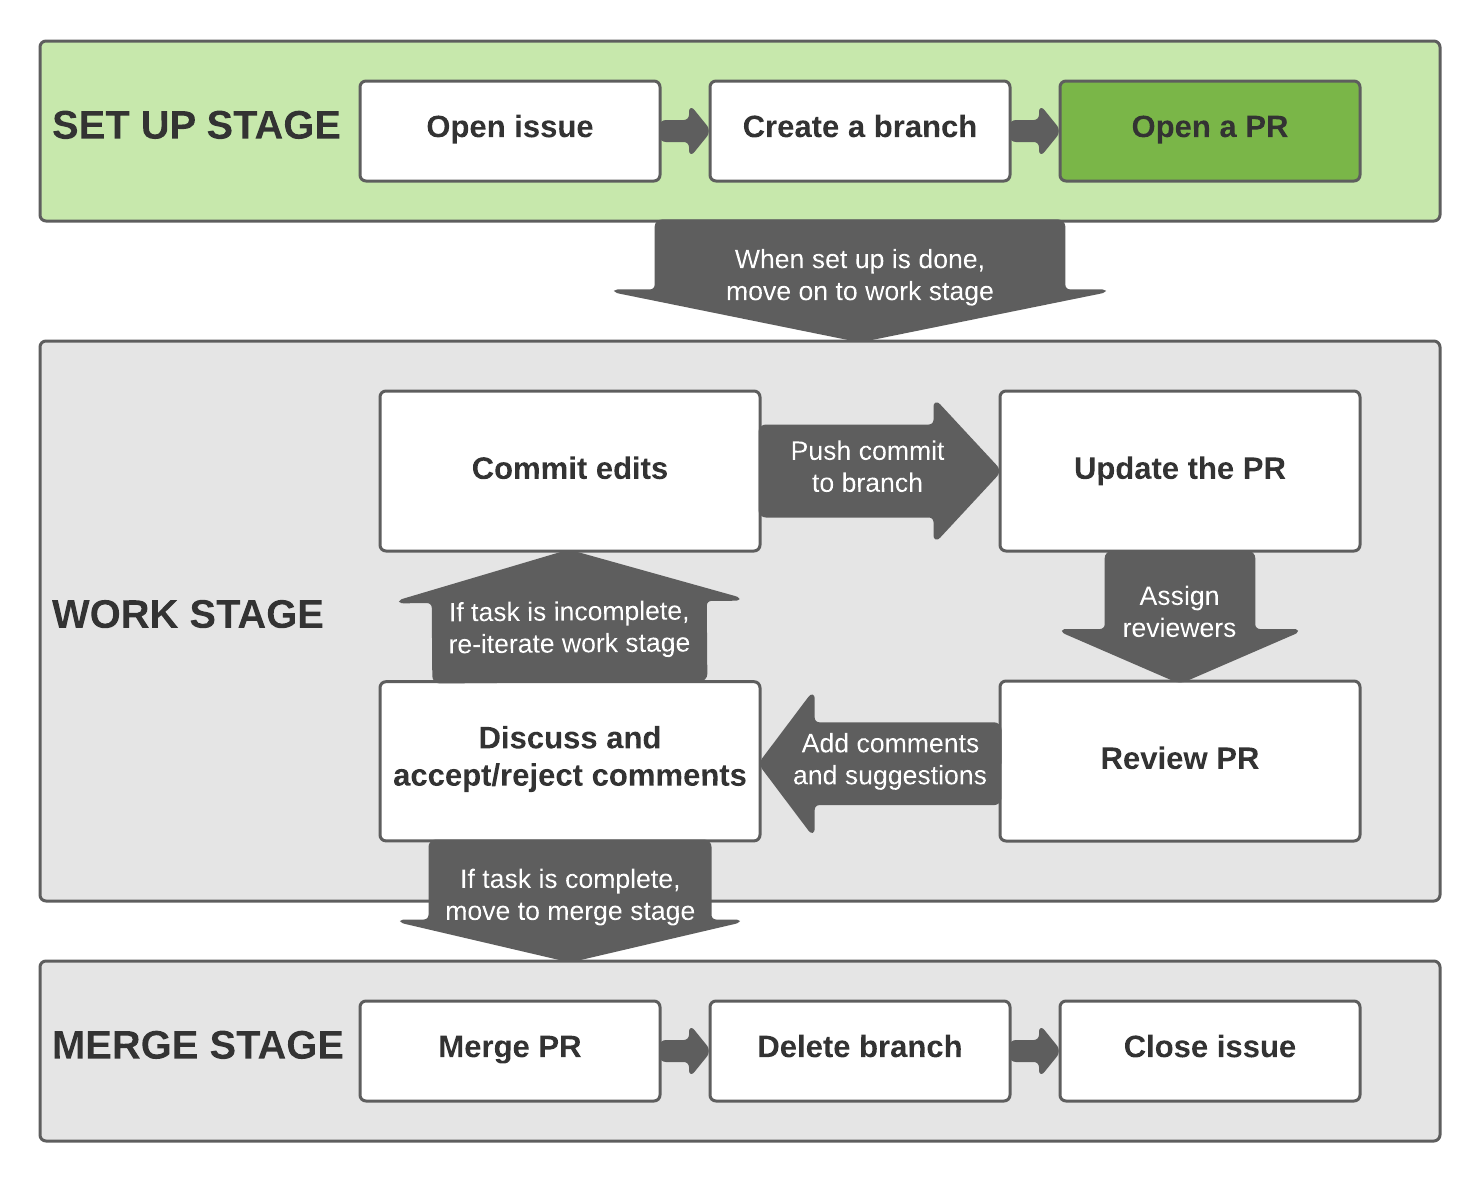
\includegraphics[width=\textwidth]{./img/branch-pr-merge-cycle-S1-3.png}
		\end{figure}
		
	\end{columns}
\end{frame}



\begin{frame}
	\frametitle{Create an draft PR}
	\begin{columns}[c]
		
		\column{.53\textwidth} % Right column and width
		\vspace{-.5cm}
		\begin{figure}
			\centering
			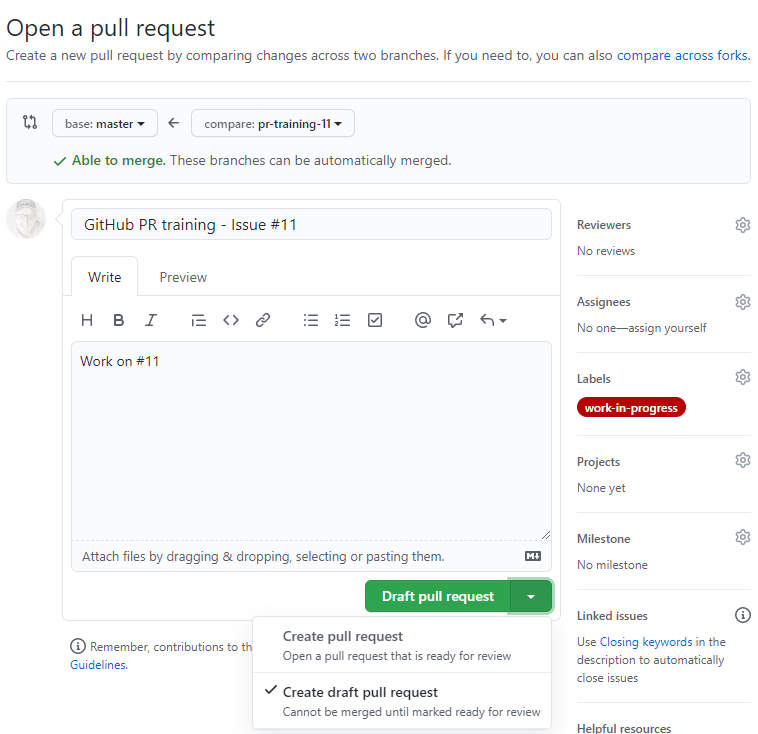
\includegraphics[width=\textwidth]{./img/create-pr-1.png}
		\end{figure}
		
		\column{.47\textwidth} % Left column and width
		
		\begin{itemize}
			\setlength\itemsep{.5em}
			\item Give the PR a name associated with the branch name but more descriptive
			\item Add \texttt{\#11} in the description to create a hyper link to issue - add \texttt{work-in-progress} label
			\item Click the arrow on the green button and select \textit{Create draft pull request}
			\item A PR cannot be merged while in draft status - signals work in progress
		\end{itemize}
		
	\end{columns}	
\end{frame}

\begin{frame}
	\frametitle{Browse draft PR}
	\begin{columns}[c]
		
		\column{.6\textwidth} % Right column and width
		\vspace{-.5cm}
		\begin{figure}
			\centering
			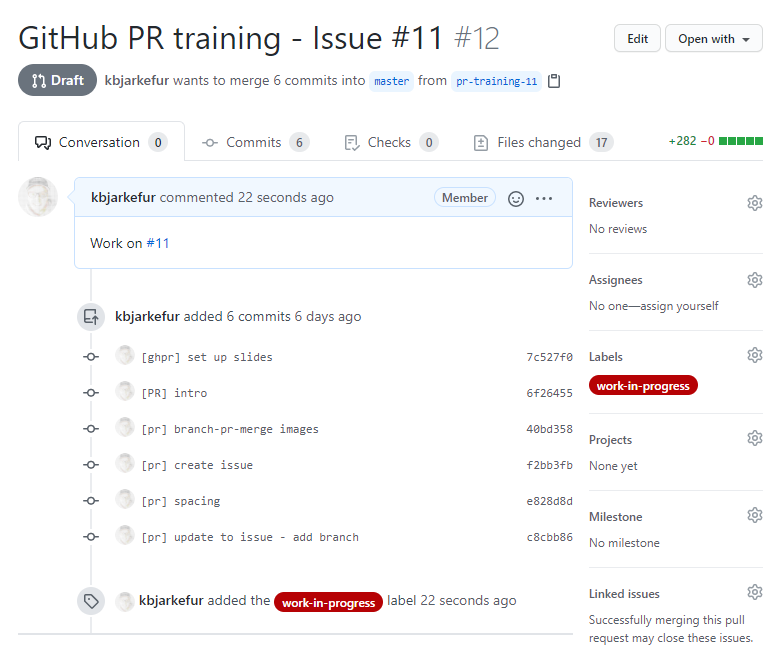
\includegraphics[width=\textwidth]{./img/create-pr-2.png}
		\end{figure}
		
		\column{.4\textwidth} % Left column and width
		
		\begin{itemize}
			\setlength\itemsep{1em}
			\item A draft PR has the color code gray 
			\item You can follow someone's work here - but no one is required to review anything yet
			\item The author will eventually remove the draft status and ask for reviews
		\end{itemize}
		
	\end{columns}	
\end{frame}

\begin{frame}
	\frametitle{Stage: The work stage}
	
	\huge\centering \textbf{WORK STAGE}
	
\end{frame}

\begin{frame}
	\frametitle{Stage: The work stage}
	\begin{columns}[c]
		
		\column{.35\textwidth} % Left column and width
		
		\Large \textbf{The work stage:}
		\vspace{.5em}
		\normalsize
		\begin{itemize}
			\setlength\itemsep{.5em}
			\item Most time will be spent in this stage
			\item Reviewing the code should be seen as a step as important as writing it
			\item This stage will be repeated until the team agrees on the quality of the code
		\end{itemize}
		
		\column{.65\textwidth} % Right column and width
		\vspace{-.75cm}
		\begin{figure}
			\centering
			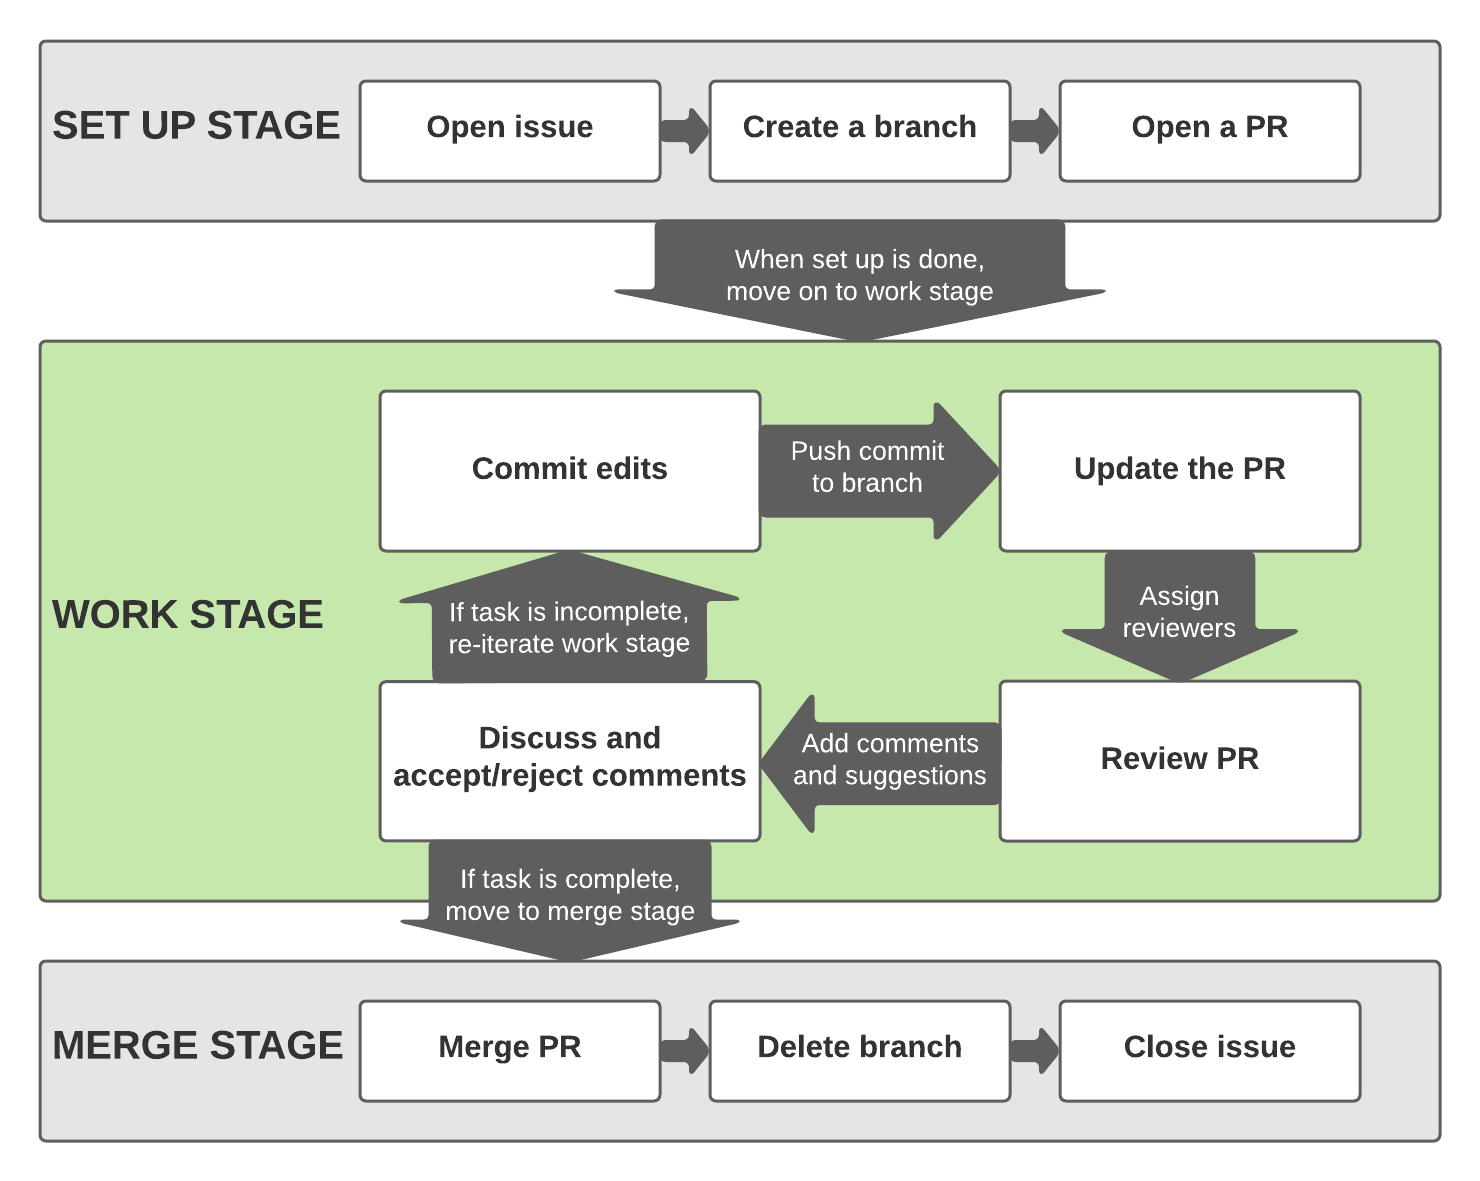
\includegraphics[width=\textwidth]{./img/branch-pr-merge-cycle-S2.png}
		\end{figure}
		
	\end{columns}
\end{frame}

\begin{frame}
	\frametitle{Make commits}
	\begin{columns}[c]
		
		\column{.35\textwidth} % Left column and width
		\begin{itemize}
			\setlength\itemsep{1em}
			\item The author commits edits as usual
			\item The draft PR will be updated as more commits are pushed to the branch		
			\item Keep pushing commits until the first implementation of the task is complete
		\end{itemize}
		
		\column{.65\textwidth} % Right column and width
		\vspace{-.75cm}
		\begin{figure}
			\centering
			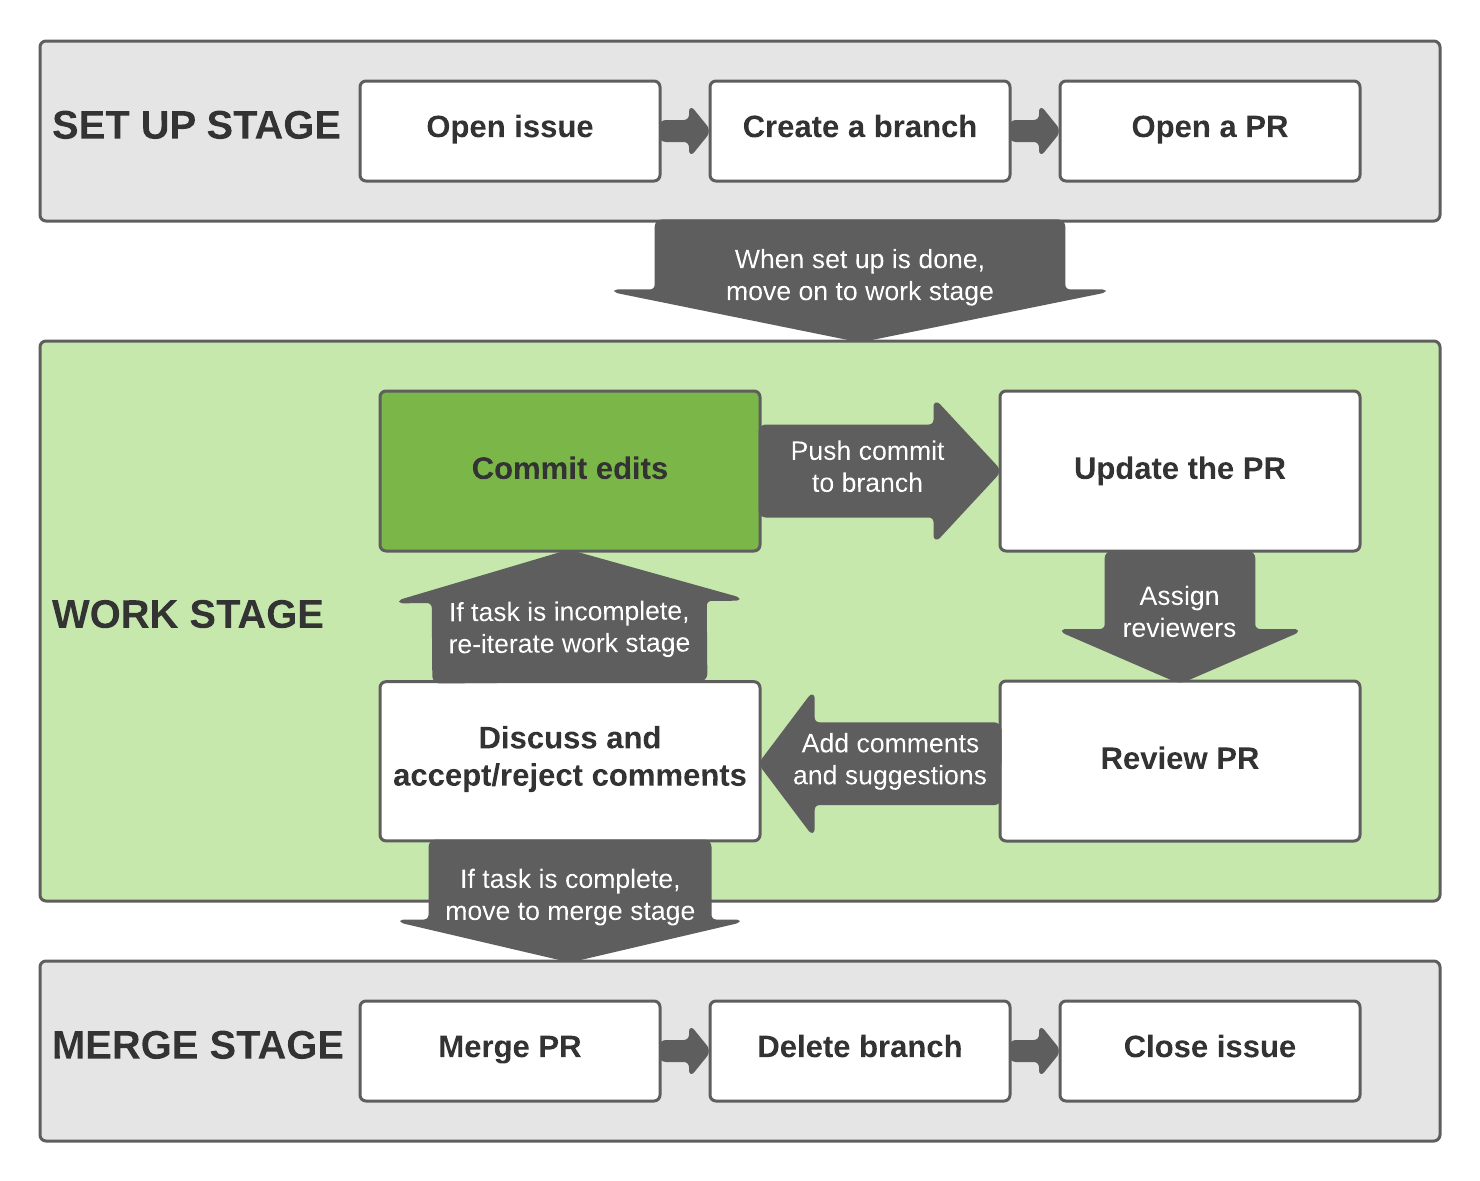
\includegraphics[width=\textwidth]{./img/branch-pr-merge-cycle-S2-1.png}
		\end{figure}
		
	\end{columns}
\end{frame}

\begin{frame}
	\frametitle{Update the PR}
	\begin{columns}[c]
		
		\column{.35\textwidth} % Left column and width
		\begin{itemize}
			\setlength\itemsep{1em}
			\item Remove the draft status from the PR
			\item Document what has been implemented in the PR
			\item Assign one or several people to review your PR
			\item Notify the assignee(s) using email or slack as GitHub notifications may be muted
		\end{itemize}
		
		\column{.65\textwidth} % Right column and width
		\vspace{-.75cm}
		\begin{figure}
			\centering
			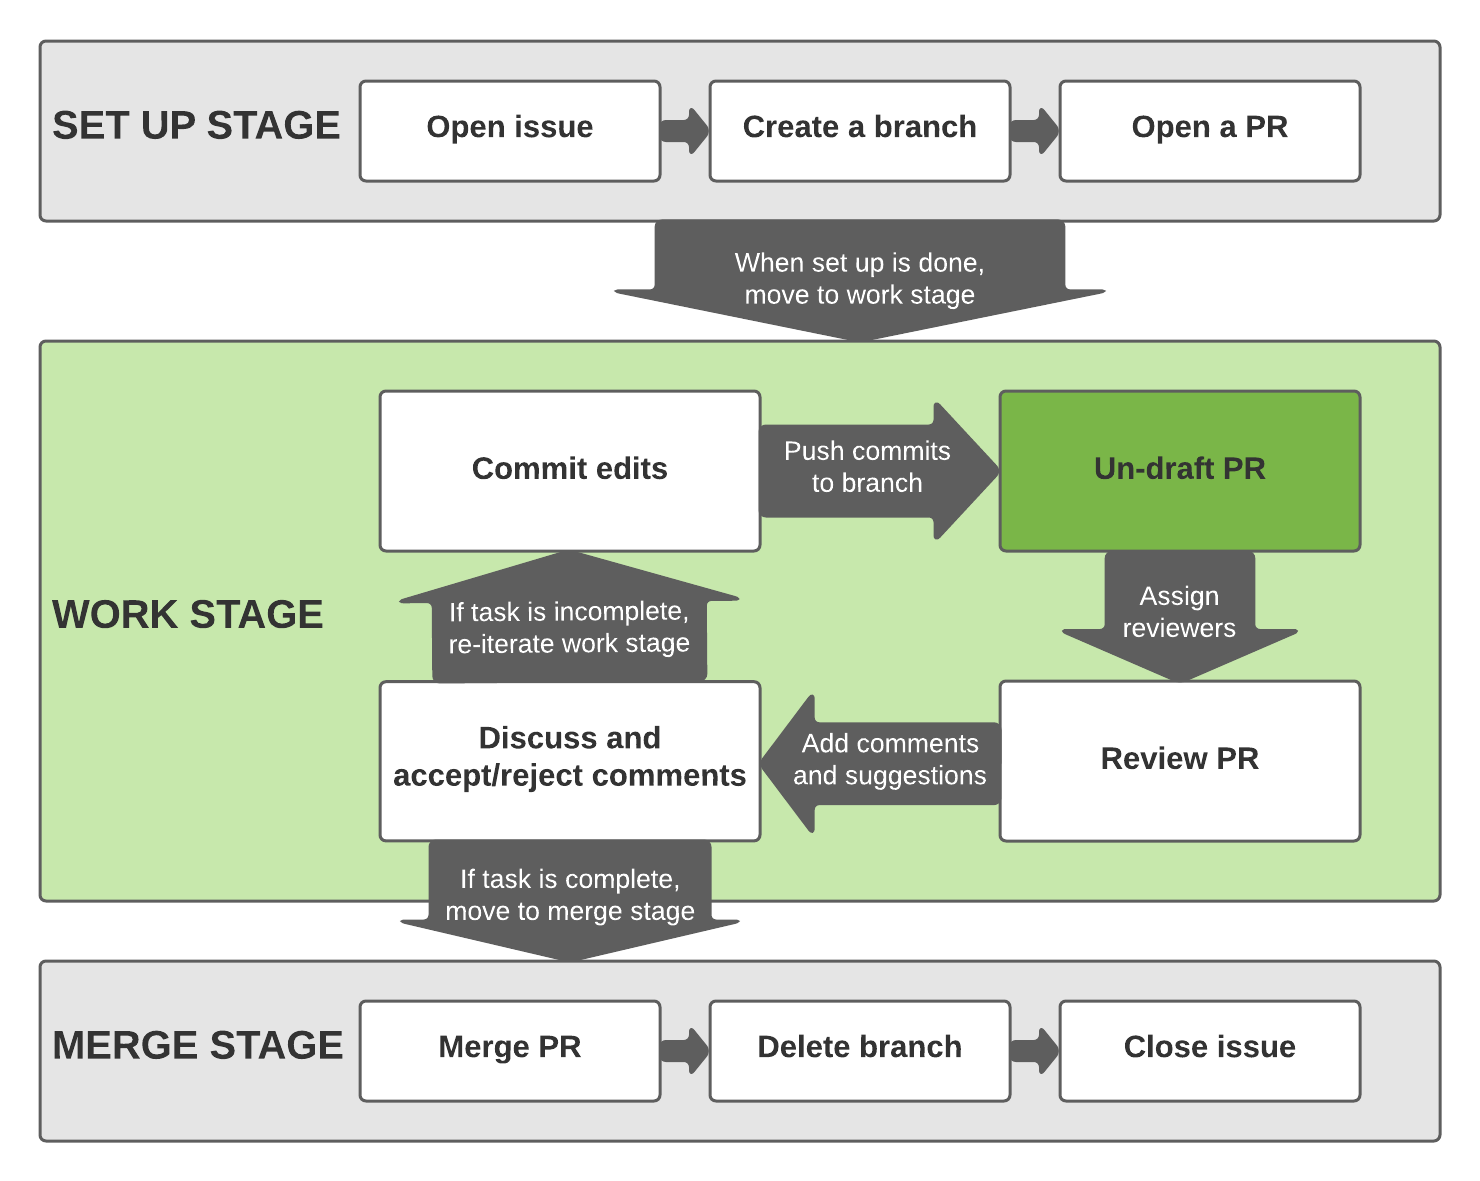
\includegraphics[width=\textwidth]{./img/branch-pr-merge-cycle-S2-2.png}
		\end{figure}
		
	\end{columns}
\end{frame}

\begin{frame}
	\frametitle{Review the PR}
	\begin{columns}[c]
		
		\column{.35\textwidth} % Left column and width
		\begin{itemize}
			\setlength\itemsep{1em}
			\item This step is incredibly important for high-quality code
			\item Use the PR to review code edits in the \textit{file changes} tab
			\item The reviewer adds code suggestions and comments
		\end{itemize}
		
		\column{.65\textwidth} % Right column and width
		\vspace{-.75cm}
		\begin{figure}
			\centering
			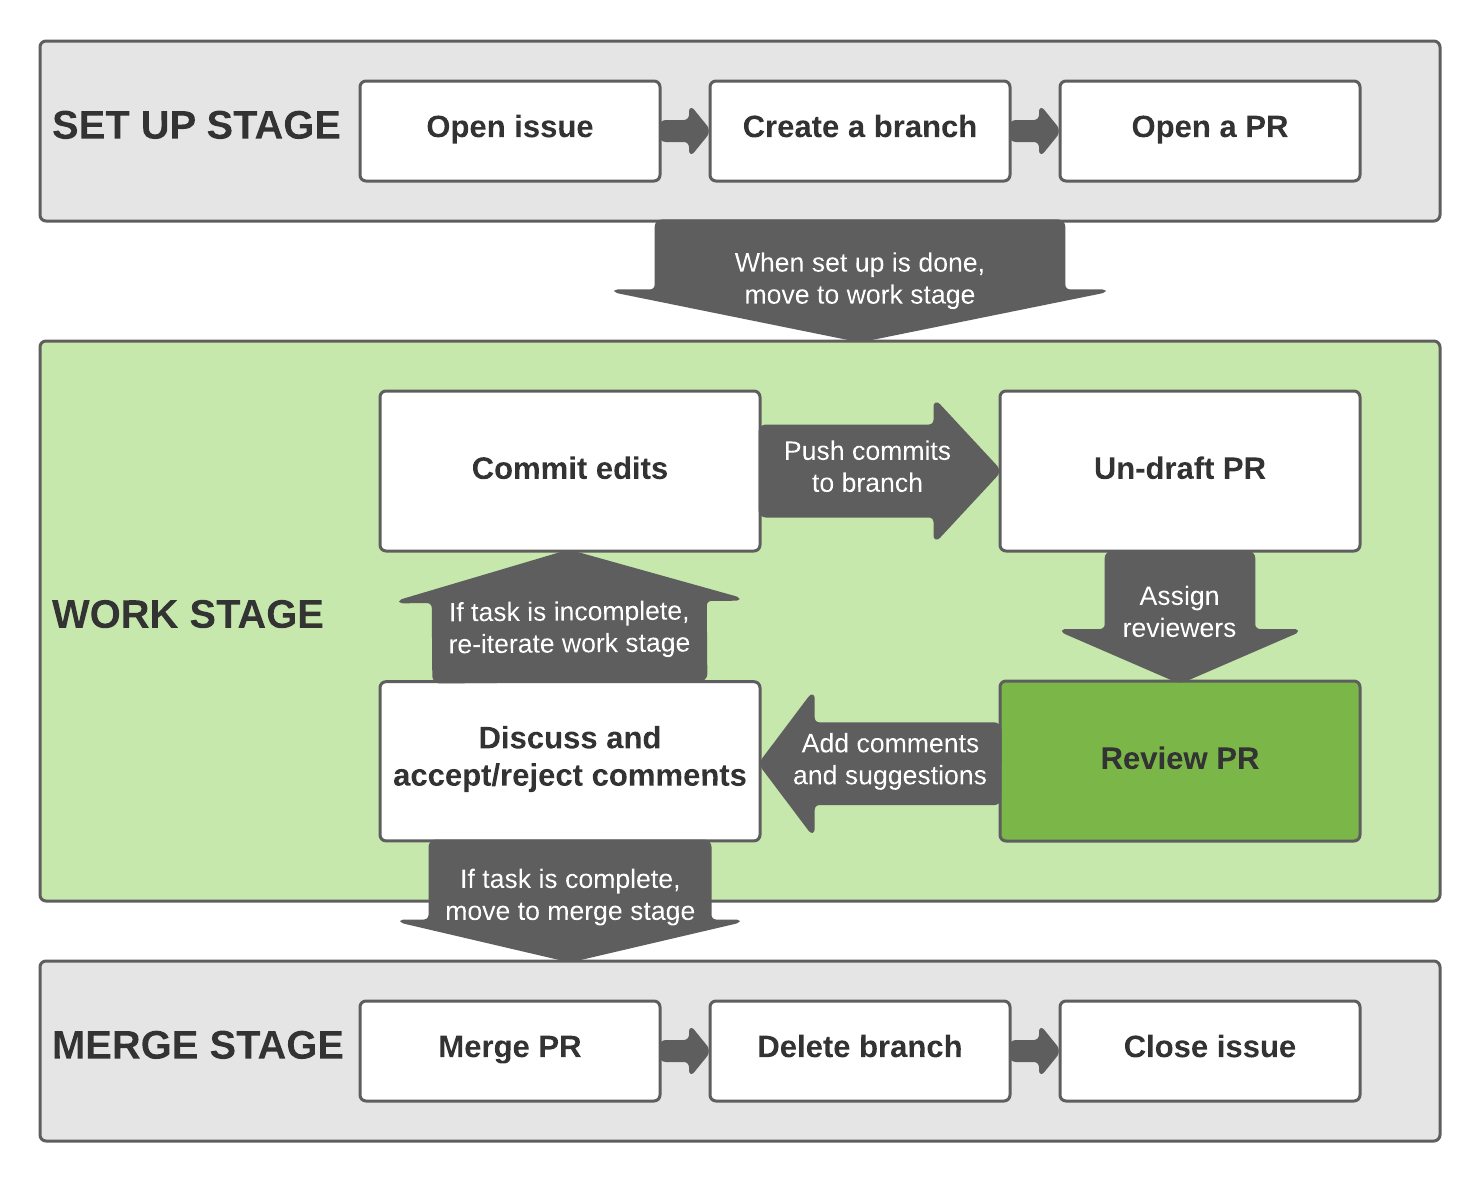
\includegraphics[width=\textwidth]{./img/branch-pr-merge-cycle-S2-3.png}
		\end{figure}
		
	\end{columns}
\end{frame}

\begin{frame}
	\frametitle{Review the PR}
	\begin{columns}[c]
	
		\column{.65\textwidth} % Right column and width
		\vspace{-.75cm}
		\begin{figure}
			\centering
			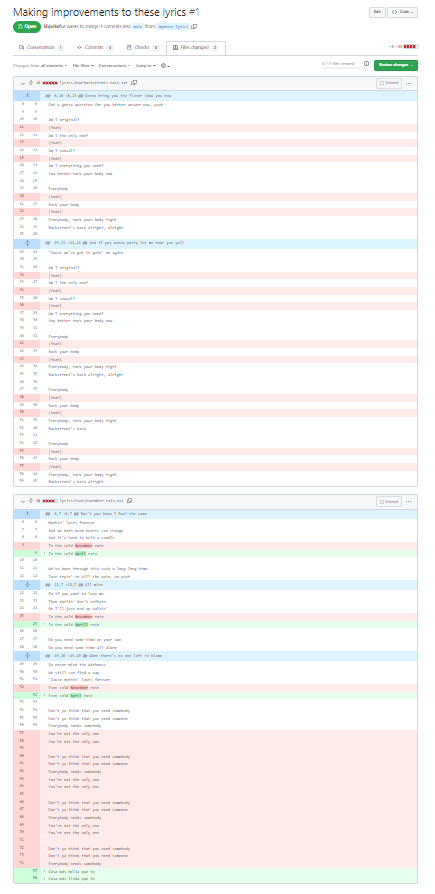
\includegraphics[width=\textwidth]{./img/review-1.png}
		\end{figure}	
		
		\column{.35\textwidth} % Left column and width
		\begin{itemize}
			\setlength\itemsep{2em}
			\item When reviewing a PR, always start by reading what the author or anyone else have written in the \textit{"Conversation"} tab
			\item Then go to the \textit{"Files changed"} tab - this is where you will review the new content of the files
		\end{itemize}
		
	\end{columns}
\end{frame}


\begin{frame}
	\frametitle{Line comments}
	\begin{columns}[c]
	
		\column{.50\textwidth} % Right column and width
		\vspace{-.6cm}
		\begin{figure}
			\centering
			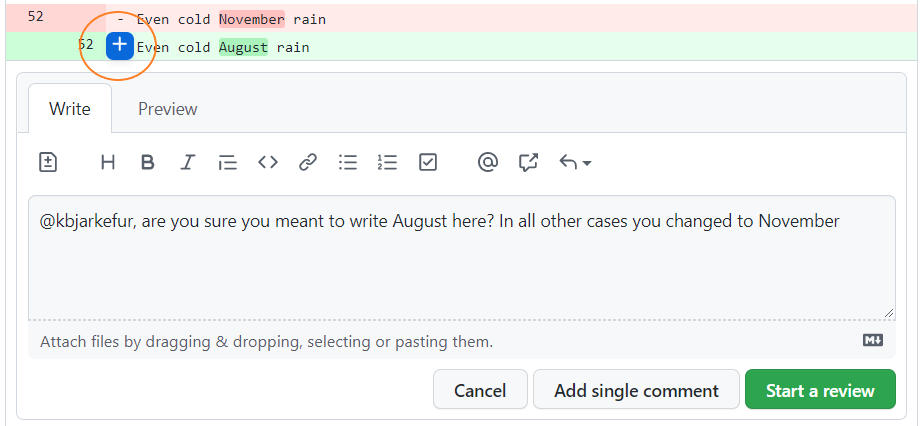
\includegraphics[width=\textwidth]{./img/line-comment-1.png}
		\end{figure}
		\vspace{-.3cm}
		\begin{figure}
			\centering
			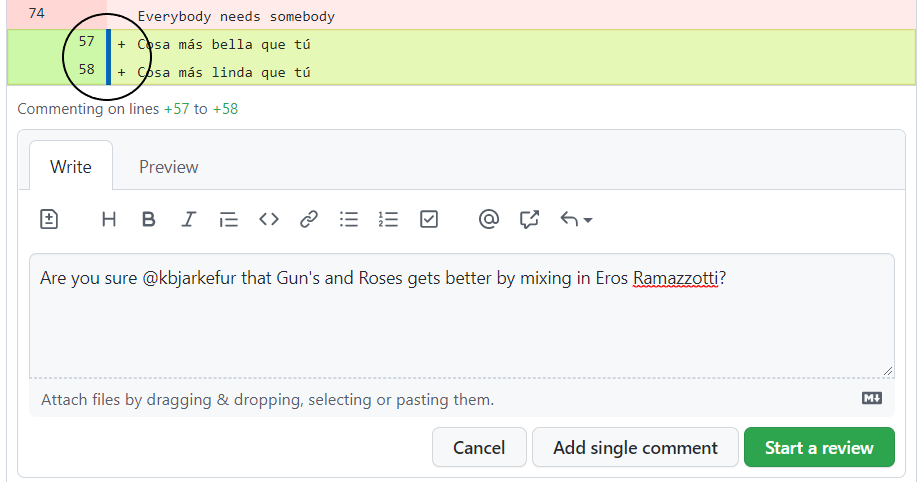
\includegraphics[width=\textwidth]{./img/line-comment-2.png}
		\end{figure}
		
		\column{.50\textwidth} % Left column and width
		\begin{itemize}
			\setlength\itemsep{.74em}
			\item Make comment on specific lines of as much as possible
			\item Click plus sign in blue circle to comment on a line 
			\item Hold shift when click and drag mouse to comment multiple lines
		\end{itemize}
	
	\end{columns}
\end{frame}

\begin{frame}
	\frametitle{Line suggestions}
	\begin{columns}[c]

		\column{.50\textwidth} % Right column and width
		\vspace{-.6cm}
		\begin{figure}
			\centering
			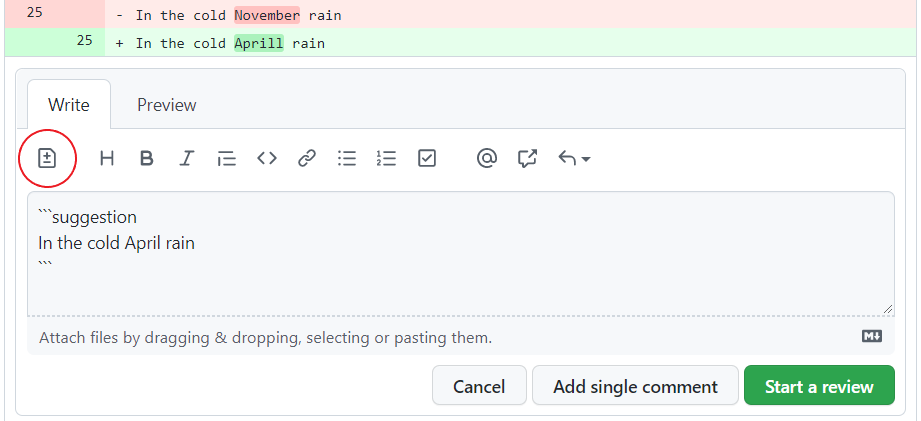
\includegraphics[width=\textwidth]{./img/suggestion-1.png}
		\end{figure}
		\vspace{-.3cm}
		\begin{figure}
			\centering
			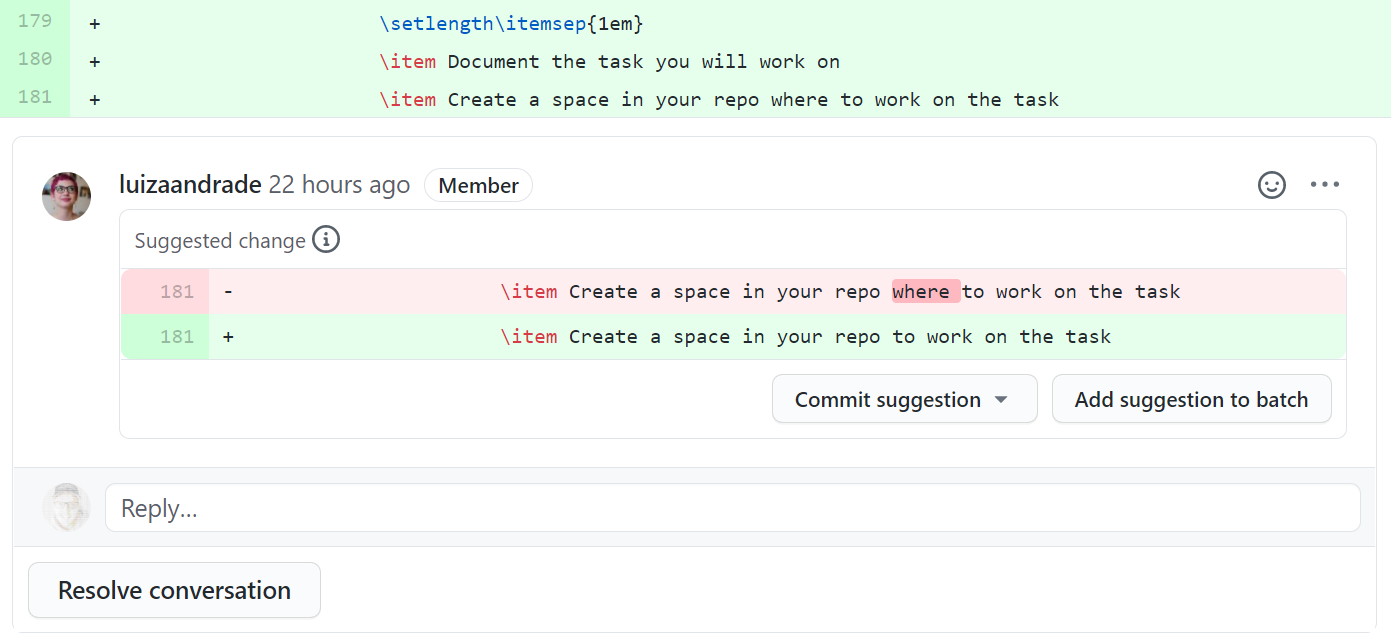
\includegraphics[width=\textwidth]{./img/suggestion-2.png}
		\end{figure}
		
		\column{.50\textwidth} % Left column and width
		\begin{itemize}
			\setlength\itemsep{.74em}
			\item You can also suggest an edit directly to the code if the edit is not too big
			\item Click the suggestion button (red circle), and edit the line
			\item The author will then see the edit that you are suggesting
			\item Can be done in multi line comments too
		\end{itemize}
		
	\end{columns}
\end{frame}

\begin{frame}
	\frametitle{PR comments}
	\begin{columns}[c]
		
		\column{.6\textwidth} % Right column and width
		\vspace{-.75cm}
		\begin{figure}
			\centering
			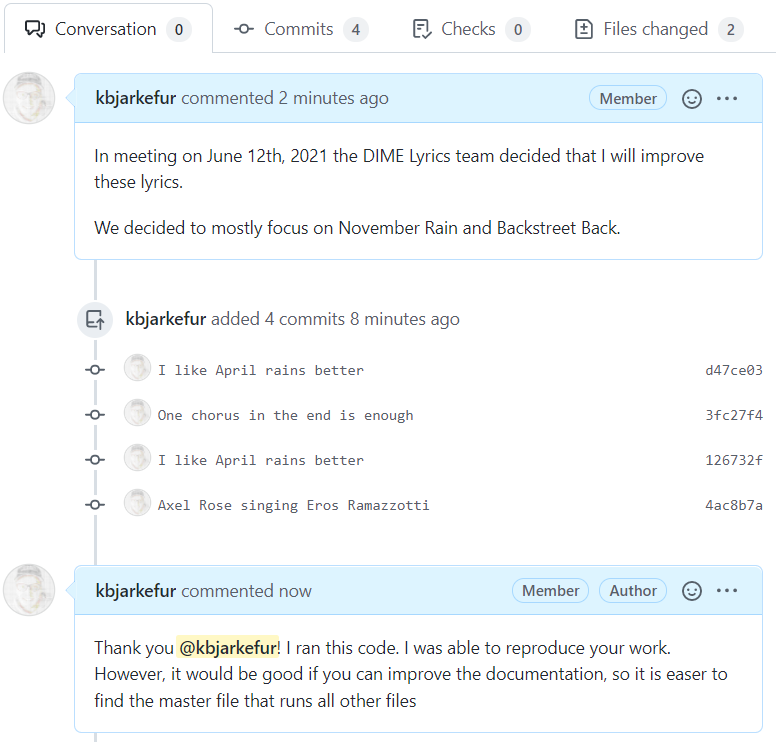
\includegraphics[width=\textwidth]{./img/pr-comment.png}
		\end{figure}	
		
		\column{.4\textwidth} % Left column and width
		\begin{itemize}
			\setlength\itemsep{1em}
			\item Make overall comments and comments that cannot be done to a specific section of the code in thread in the \textit{"Conversation"} tab
			\item Suggestions are also listed here
			\item Tag the author so they get a notification that someone have reviewed the PR
		\end{itemize}
		
	\end{columns}
\end{frame}

\begin{frame}
	\frametitle{Discuss and accept/reject}
	\begin{columns}[c]
		
		\column{.35\textwidth} % Left column and width
		\begin{itemize}
			\setlength\itemsep{1em}
			\item The author accepts or discusses suggestions and replies to comments
			\item Then the author and the reviewers (and anyone else in the project team) come together and decide if the task is complete or not
		\end{itemize}
		
		\column{.65\textwidth} % Right column and width
		\vspace{-.75cm}
		\begin{figure}
			\centering
			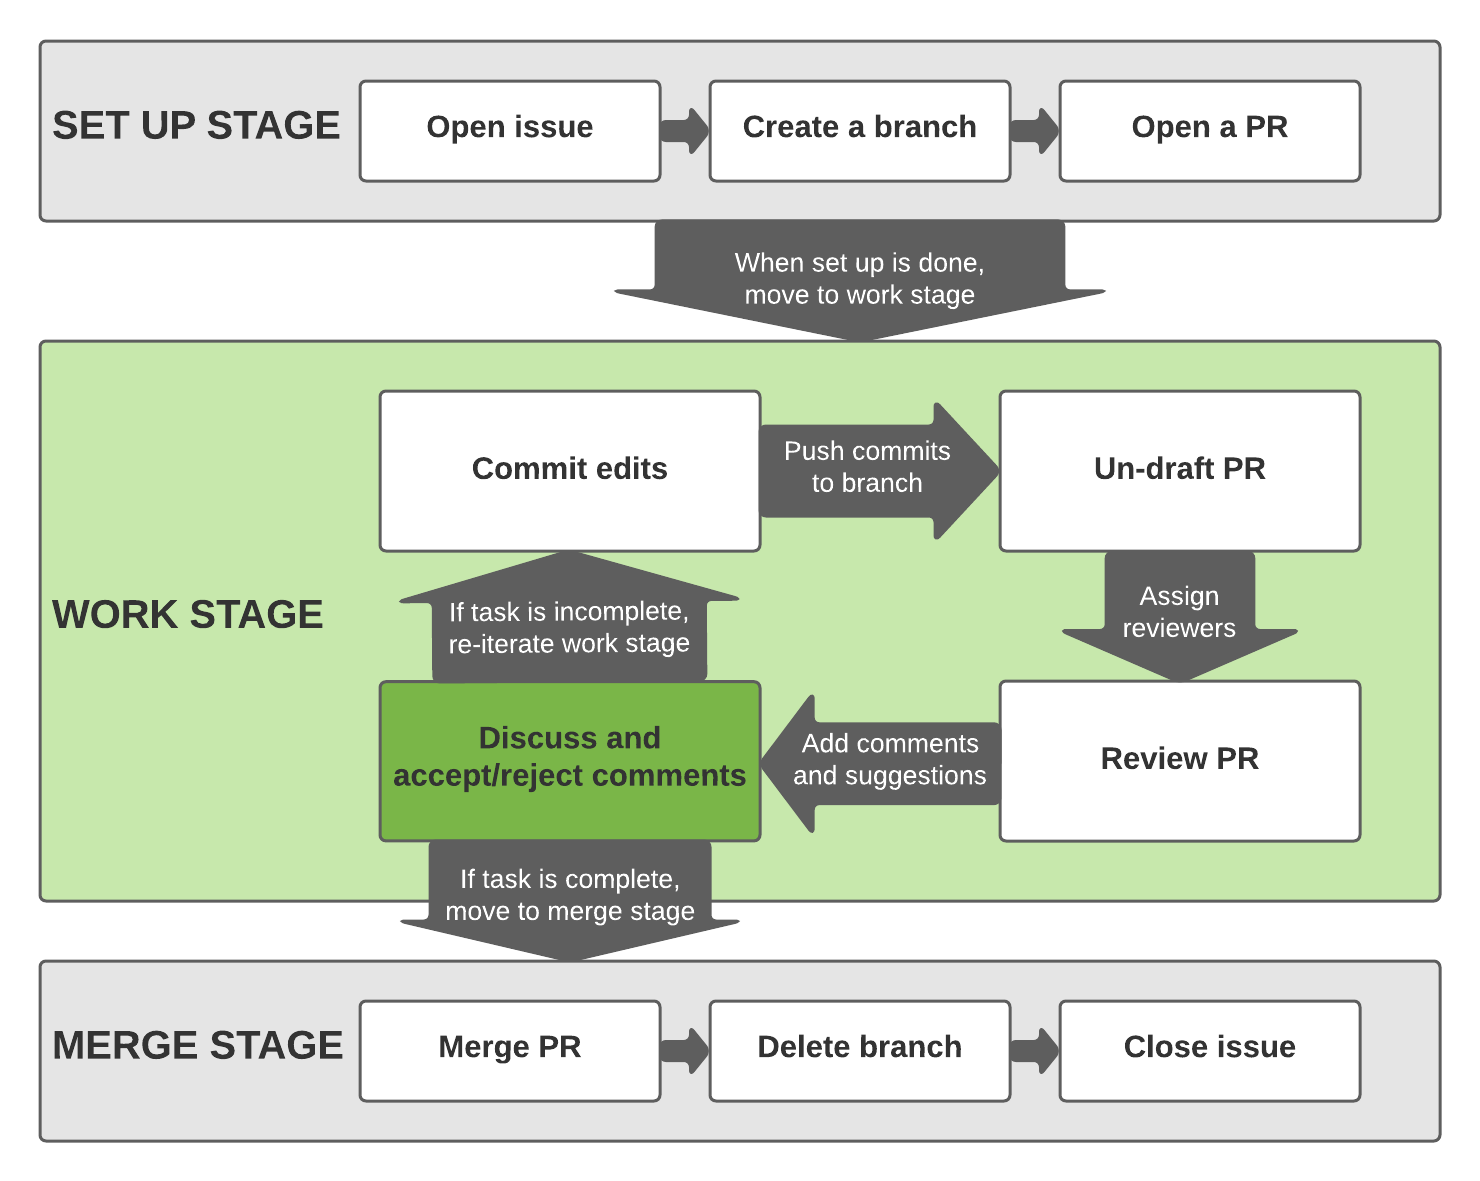
\includegraphics[width=\textwidth]{./img/branch-pr-merge-cycle-S2-4.png}
		\end{figure}
		
	\end{columns}
\end{frame}

\begin{frame}
	\frametitle{Review suggestion}
	\begin{columns}[c]
		
		\column{.5\textwidth} % Right column and width
		\vspace{-.75cm}
		\begin{figure}
			\centering
			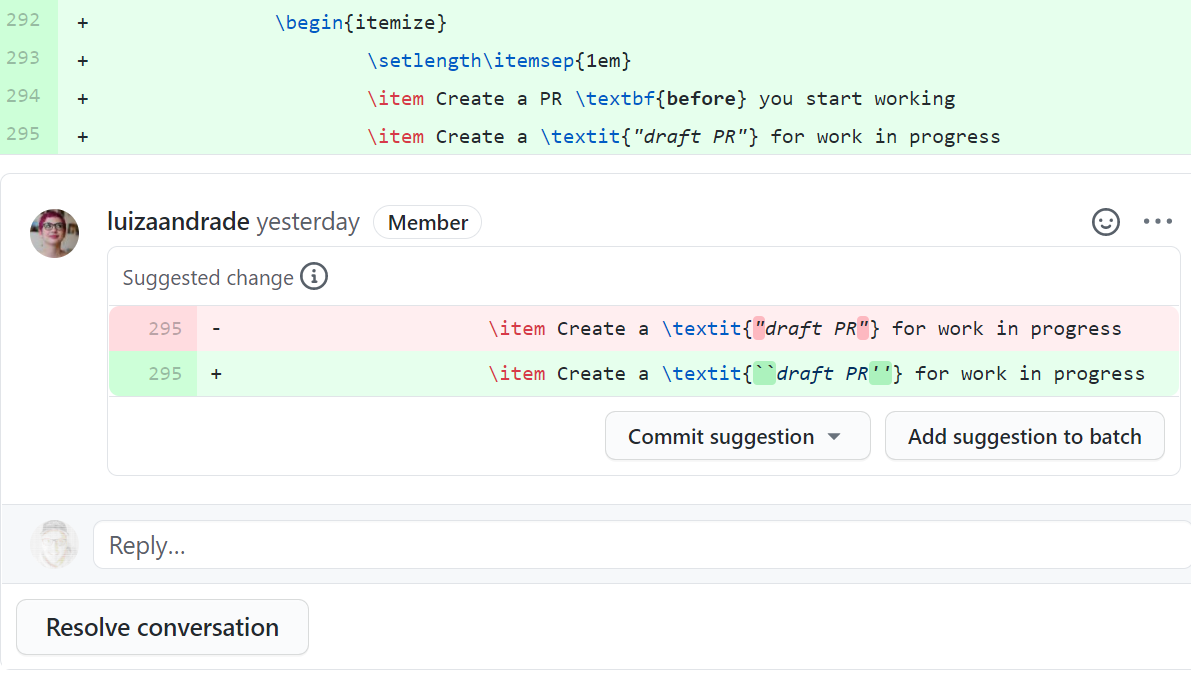
\includegraphics[width=\textwidth]{./img/review-suggestion-1.png}
		\end{figure}	
		
		\column{.5\textwidth} % Left column and width
		\begin{itemize}
			\setlength\itemsep{1em}
			\item Start by going over the suggestions as they tend to be quick  
			\item Suggestions are ordered chronologically in the \textit{"Conversation"} tab and by line number in the \textit{"File changes"} tab
			\item Accept the suggestion with \textit{Commit Suggestion}, ignore/delete it with \textit{Resolve conversation} or comment to ask for more information
		\end{itemize}
		
	\end{columns}
\end{frame}

\begin{frame}
	\frametitle{Review suggestion}
	\begin{columns}[c]
		
		\column{.35\textwidth} % Right column and width
		\Large ADD SOME ICON FOR QUALITY CONTROL
		
		\column{.65\textwidth} % Left column and width
		\begin{itemize}
			\setlength\itemsep{1em}
			\item Address all suggestions and comments until they are all done answered
			\item If major work is still required, put the PR in draft status again and add back the \textit{work-in-progress} label and start over the work stage
			\item Once there are no more small or major comments or suggestions left to do, then move on to the merge stage
		\end{itemize}
		
	\end{columns}
\end{frame}


\begin{frame}
	\frametitle{Stage: The merge stage}
	
	\huge\centering \textbf{MERGE STAGE}
	
\end{frame}

\begin{frame}
	\frametitle{Stage: The merge stage}
	\begin{columns}[c]
		
		\column{.35\textwidth} % Left column and width
		
		\Large \textbf{The merge stage:}
		\vspace{1em}
		\normalsize
		\begin{itemize}
			\setlength\itemsep{.5em}
			\item Once the work stage is complete, the merge stage is quick
			\item Clean up the task and make sure it was properly documented
		\end{itemize}
		
		\column{.65\textwidth} % Right column and width
		\vspace{-.75cm}
		\begin{figure}
			\centering
			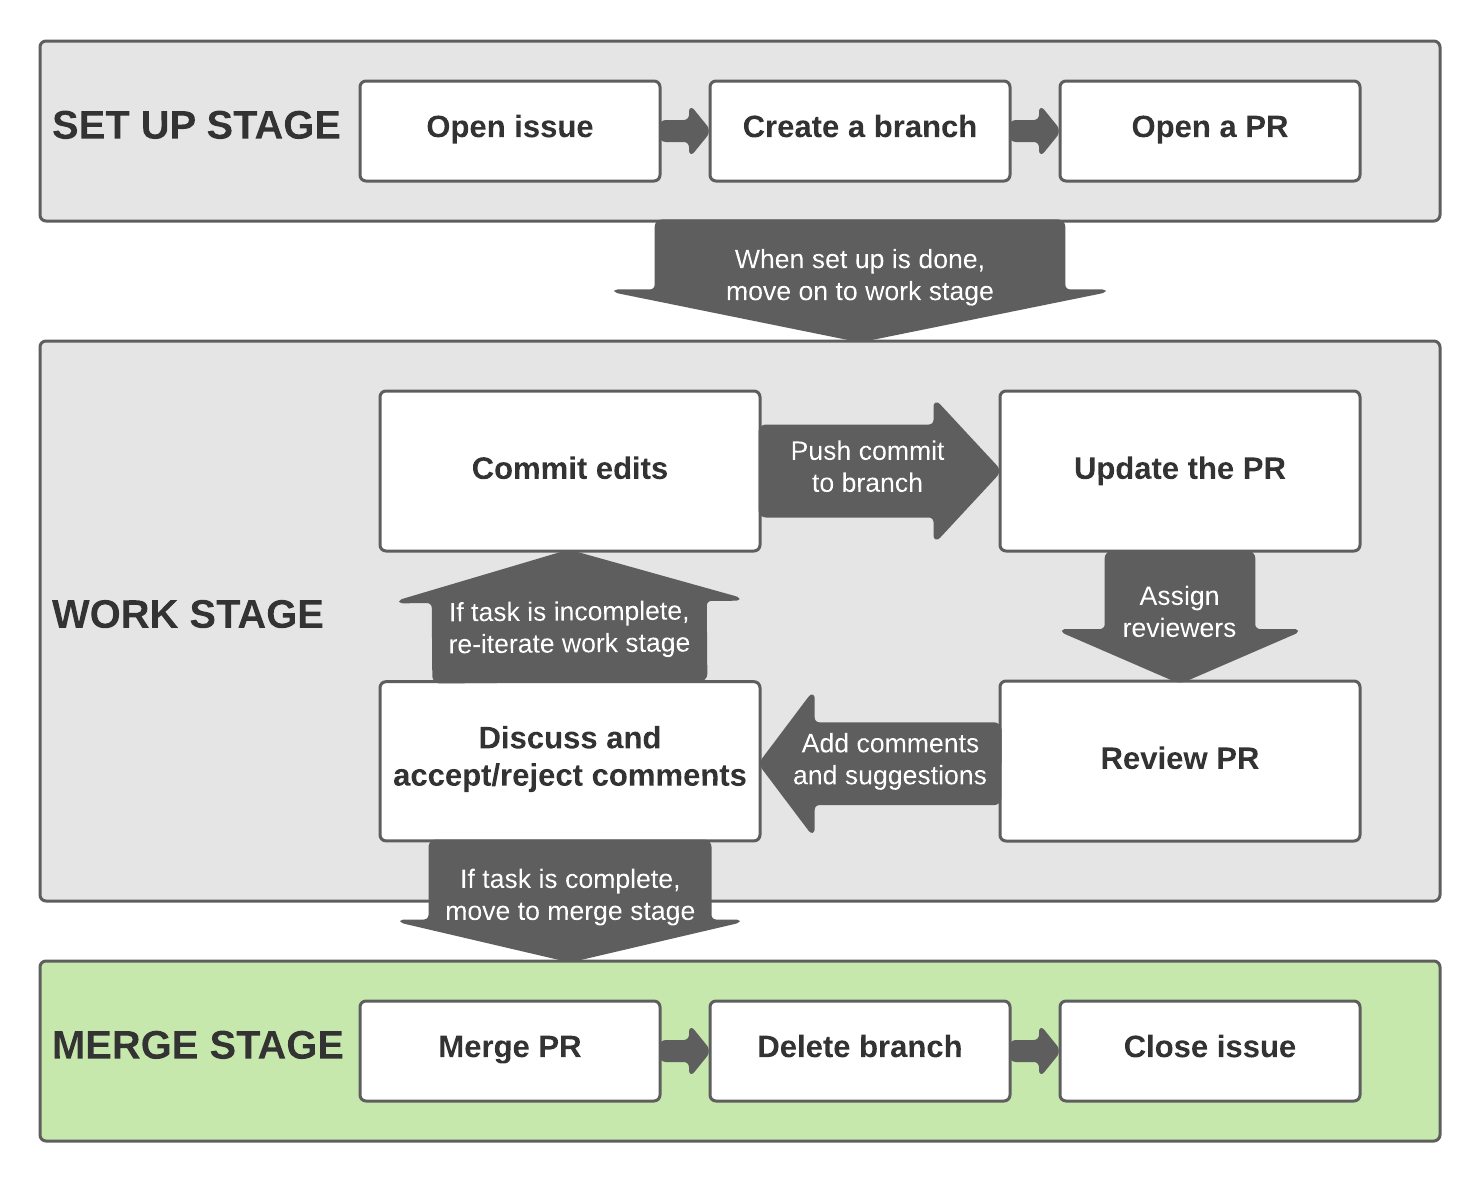
\includegraphics[width=\textwidth]{./img/branch-pr-merge-cycle-S3.png}
		\end{figure}
		
	\end{columns}
\end{frame}


\begin{frame}
	\frametitle{Merge the PR}
	\begin{columns}[c]
		
		\column{.35\textwidth} % Left column and width
		\begin{itemize}
			\setlength\itemsep{1em}
			\item Before merging, make sure that the PR is well documented - this is the most likely place a future team member will look for documentation on why tasks were implemented a certain way 
			\item Then you can merge your well-reviewed and well-documented code
			
		\end{itemize}
		
		\column{.65\textwidth} % Right column and width
		\vspace{-.75cm}
		\begin{figure}
			\centering
			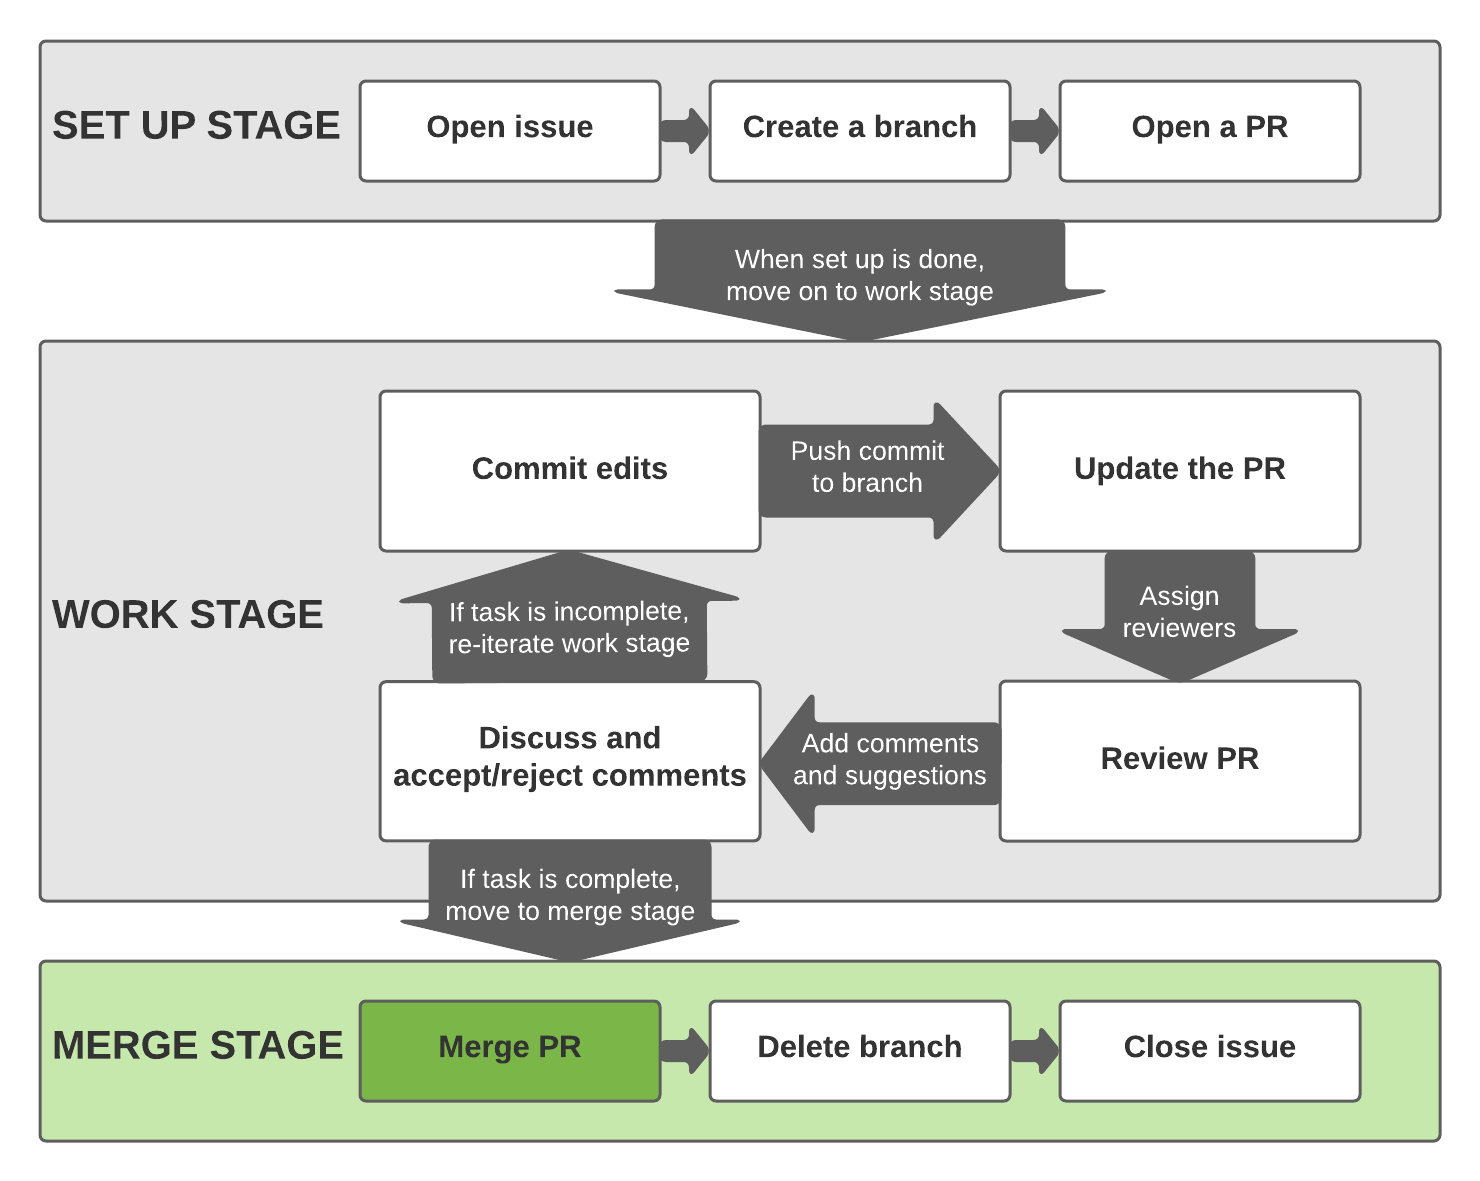
\includegraphics[width=\textwidth]{./img/branch-pr-merge-cycle-S3-1.png}
		\end{figure}
		
	\end{columns}
\end{frame}

\begin{frame}
	\frametitle{Delete the branch}
	\begin{columns}[c]
		
		\column{.35\textwidth} % Left column and width
		\begin{itemize}
			\setlength\itemsep{1em}
			\item Always delete the branch
			\item If you want to keep working in a branch with the same name, then re-create that branch
			\item Otherwise you risk working on an outdated version of the repo
		\end{itemize}
		
		\column{.65\textwidth} % Right column and width
		\vspace{-.75cm}
		\begin{figure}
			\centering
			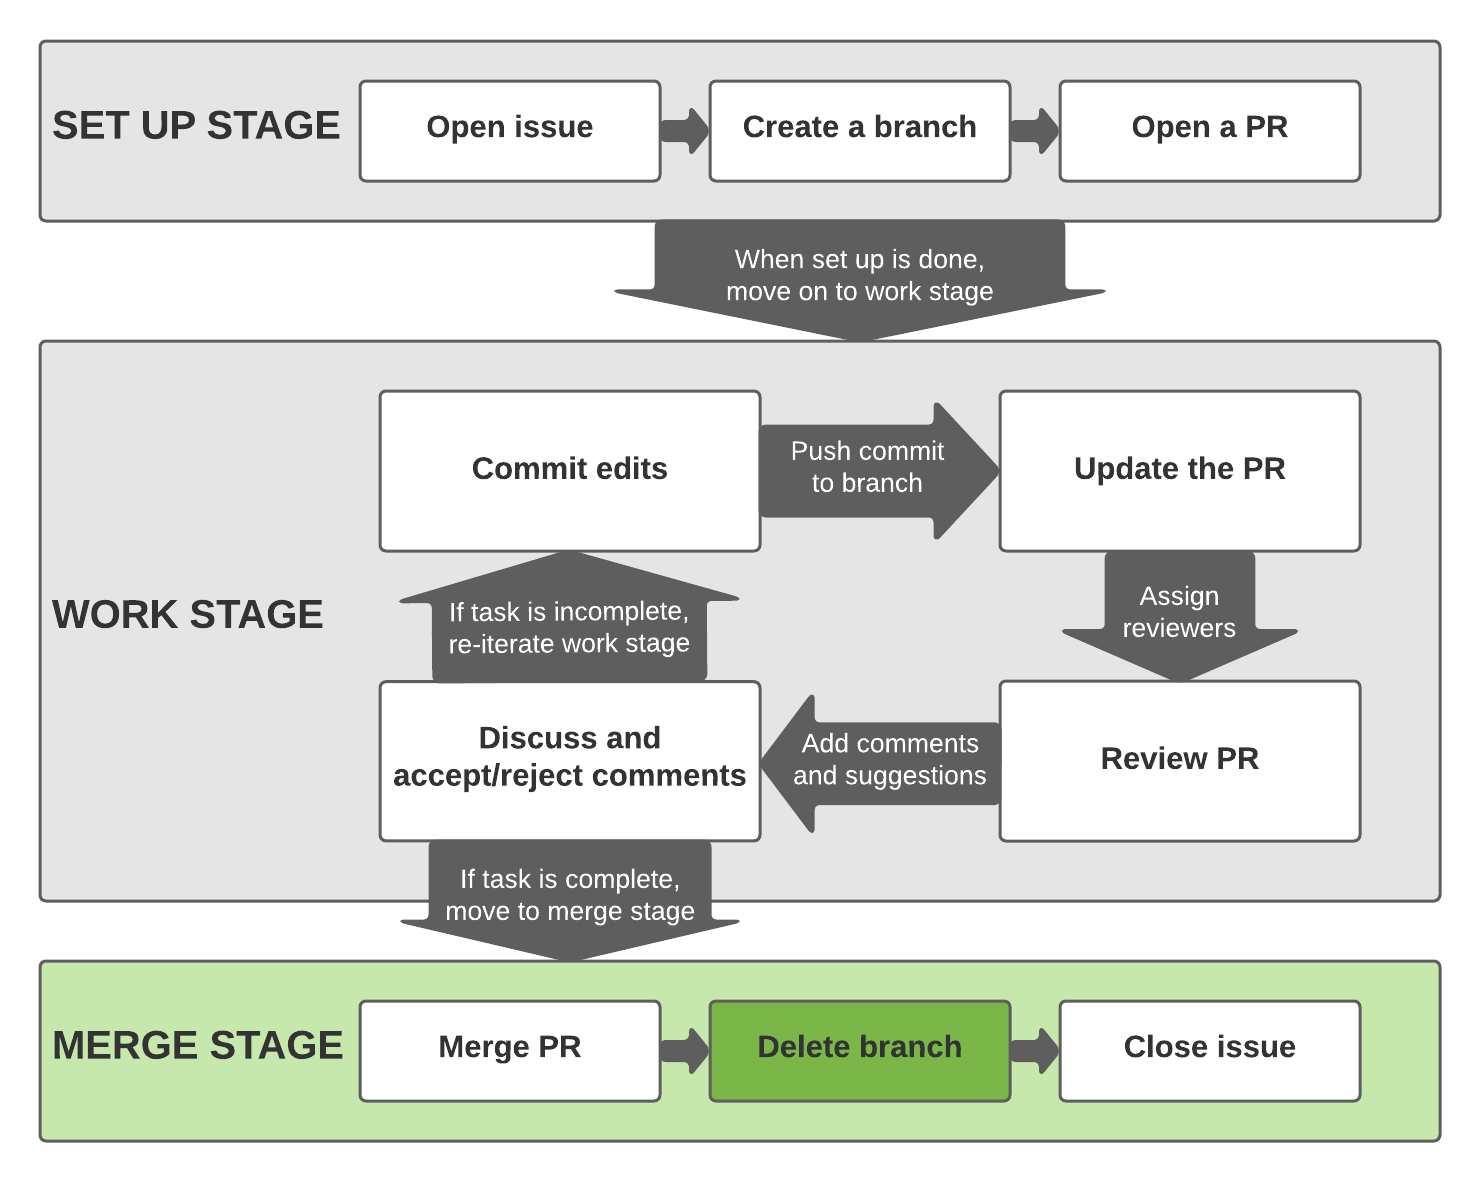
\includegraphics[width=\textwidth]{./img/branch-pr-merge-cycle-S3-2.png}
		\end{figure}
		
	\end{columns}
\end{frame}

\begin{frame}
	\frametitle{Close issue}
	\begin{columns}[c]
		
		\column{.35\textwidth} % Left column and width
		If you created an issue for this task:
		\begin{itemize}
			\setlength\itemsep{.5em}
			\item Make sure that the PR number is referenced in the issue. 
			\item For example: \textit{``Issue resolved in PR \#12''}
			\item Then close the issue
		\end{itemize}
		
		\column{.65\textwidth} % Right column and width
		\vspace{-.75cm}
		\begin{figure}
			\centering
			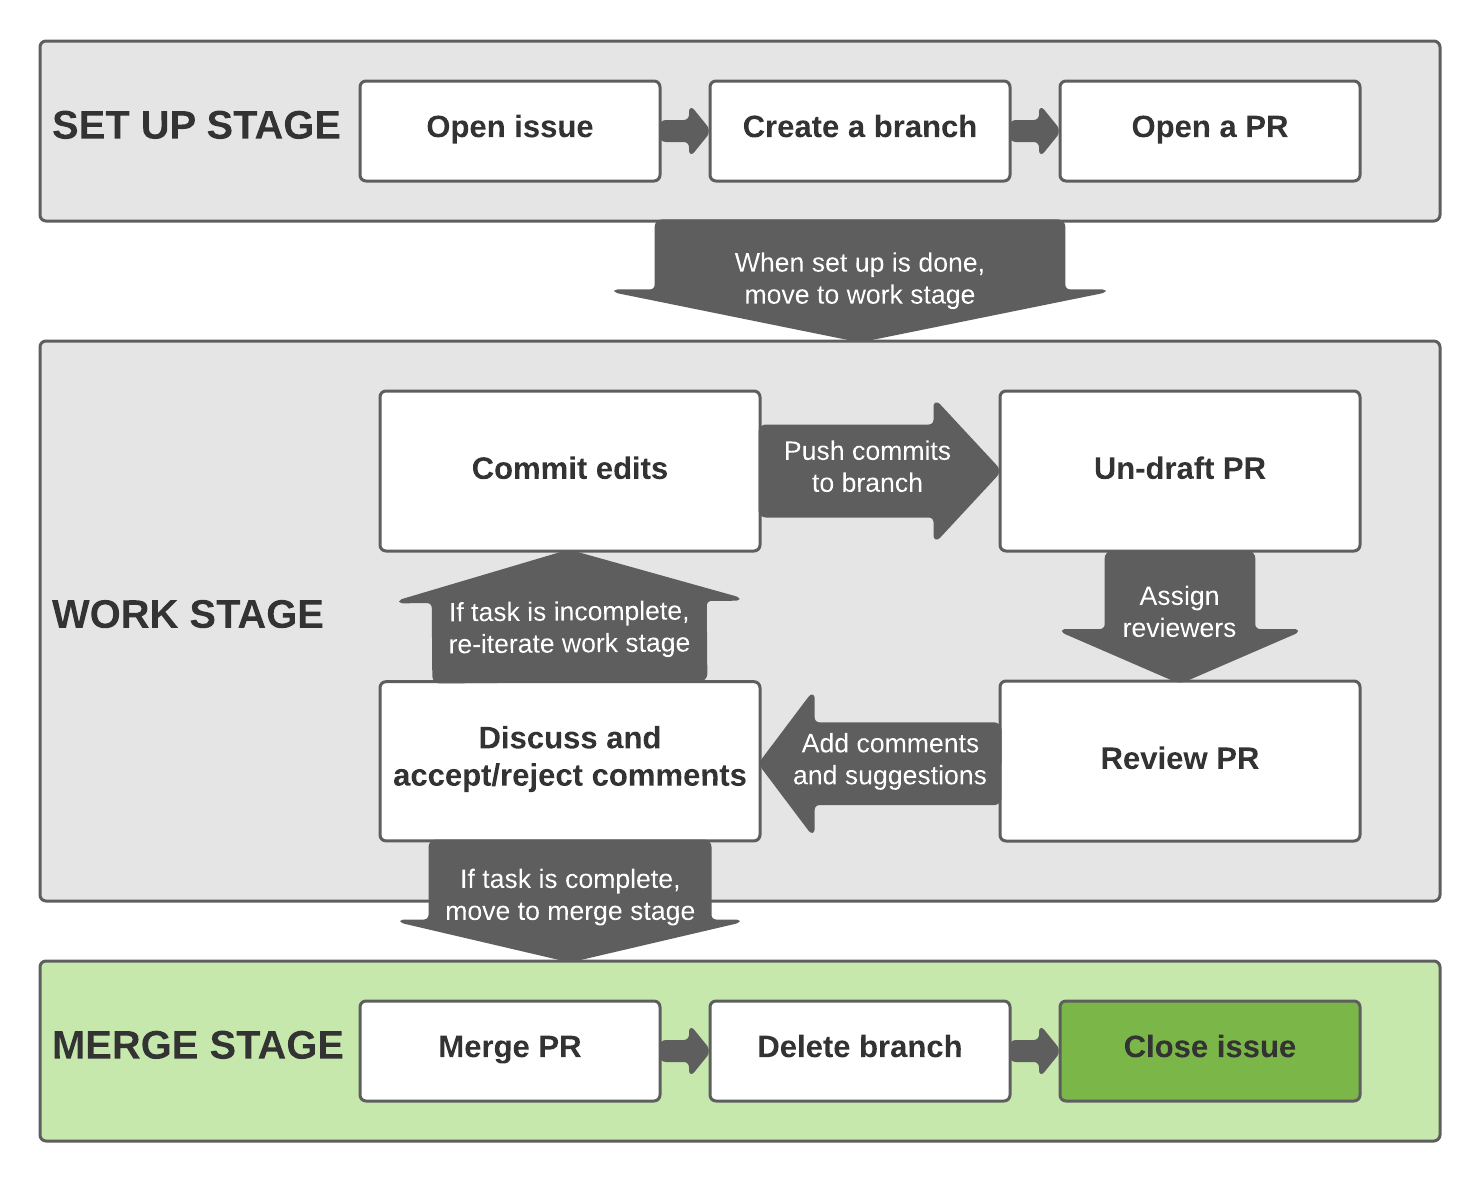
\includegraphics[width=\textwidth]{./img/branch-pr-merge-cycle-S3-3.png}
		\end{figure}
		
	\end{columns}
\end{frame}



\section{Part 2: \newline GitFlow - How to fit the ``branch-PR-merge'' cycle into your workflow}


\begin{frame}{Useful links}
	\begin{itemize}
	  \item All DIME Analytics GitHub trainings: \trainingURL{https://osf.io/e54gy/}
	  \item Other DIME Analytics GitHub resources: \trainingURL{https://github.com/worldbank/dime-github-trainings}. For example:
		\begin{itemize}
			\item DIME Analytics GitHub Templates (for example .gitignore): \trainingURL{https://github.com/worldbank/dime-github-trainings/tree/master/GitHub-resources/DIME-GitHub-Templates}
			\item DIME Analytics GitHub Roles: \trainingURL{https://github.com/worldbank/dime-github-trainings/blob/master/GitHub-resources/DIME-GitHub-Roles/DIME-GitHub-roles.md}
		\end{itemize}
		\item Markdown cheat sheet (how to format text on GitHub.com):  \trainingURL{https://www.markdownguide.org/cheat-sheet/}
		\item DIME GitHub Account admin info and instructions: \trainingURL{https://github.com/dime-worldbank/dime-account-admin}
	\end{itemize}
\end{frame}


\input{../../Common-Resources/slides/GitHub-Commit-URL.tex}


\end{document}
